% ------------------------------------------------------------------------------
% 7.3. DISEÑO DE DATOS
% ------------------------------------------------------------------------------
\subsection{7.3. Diseño de Datos}\label{sec:cap7_diseno_datos}

El diseño de datos traduce las clases persistentes del diagrama de clases (sección~\ref{sec:cap7_diagrama_clase}) a un modelo relacional implementado en PostgreSQL. El modelo consta de 31 tablas agrupadas según los seis paquetes del análisis: Cuentas y acceso (4), Convocatoria y postulación (9), Preselección con IA (4), Auditoría y adjudicación (8), Becados y asistencia (5) y Reportes y trazabilidad (1). Los nombres de tablas y columnas se escriben en minúsculas, en singular y separados por guion bajo; cada tabla tiene una clave primaria interna \textit{id} y las claves foráneas se nombran \textit{\textless{}tabla\textgreater{}\_id}.

Todas las tablas incorporan cuatro columnas comunes: \textit{codigo\_\textless{}tabla\textgreater{}}, un identificador público UUID versión 7, único y no nulo, que es el único identificador que se expone a la API y a los clientes web y móvil; \textit{creado\_en} y \textit{actualizado\_en}, que registran la fecha y hora de creación y de la última modificación; y \textit{eliminado\_en}, que implementa el borrado lógico, de modo que ningún registro se elimina físicamente. Las contraseñas no se almacenan en la base de datos, pues las gestiona Firebase Authentication, y los archivos se guardan en Firebase Storage, del que la base de datos solo conserva la ruta.

\subsubsection{7.3.1. Diseño de Datos Lógico}\label{sec:cap7_datos_logico}

\paragraph{7.3.1.1. Diseño lógico de la Base de Datos.}\label{sec:cap7_logico_bd}
El diseño lógico de la base de datos representa cada tabla con sus columnas, tipos de datos, claves primarias (PK), claves foráneas (FK) y restricciones de unicidad (UQ), así como las relaciones y cardinalidades entre las tablas. La Figura~\ref{fig:diseno_logico_bd} presenta el diagrama del diseño lógico.

\begin{figure}[H]
\caption{Diseño lógico de la base de datos}
\label{fig:diseno_logico_bd}
\centering
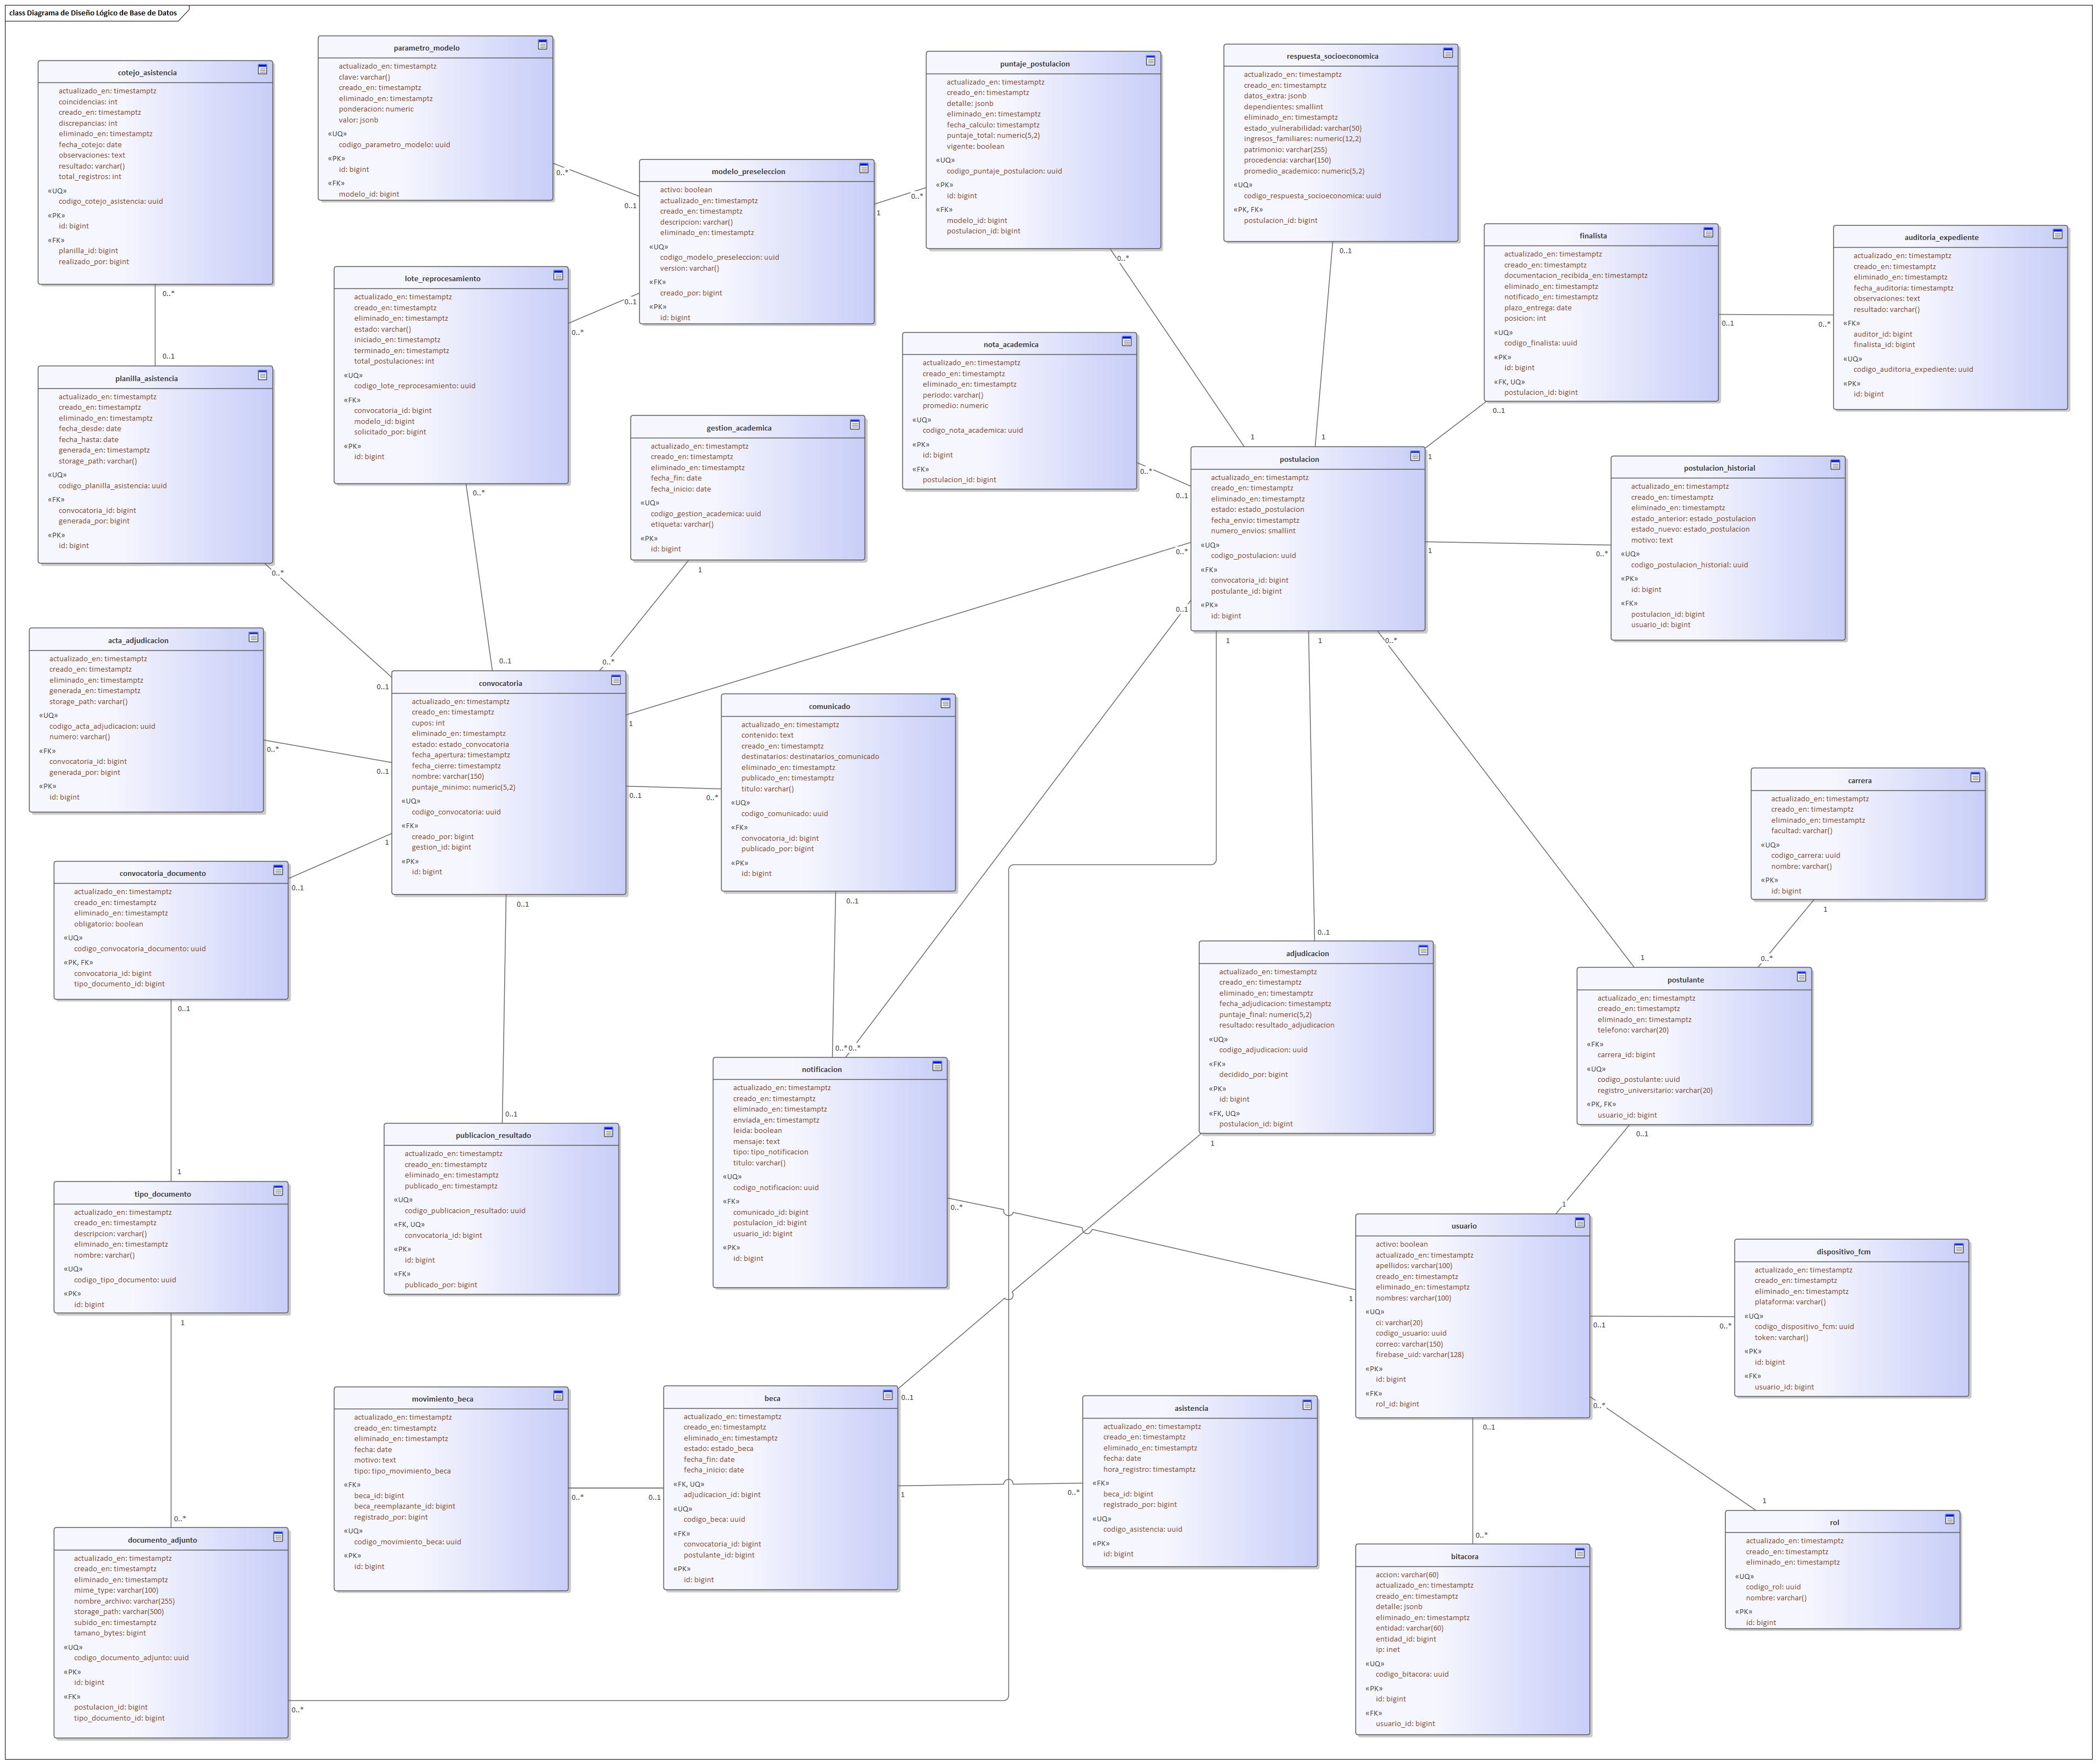
\includegraphics[width=\textwidth,height=0.8\textheight,keepaspectratio]{images/091_Diseno_Logico_Base_de_Datos.jpg}

\smallskip
\noindent\raggedright\textit{Nota.} Elaboración propia.
\end{figure}

\paragraph{7.3.1.2. Mapeo.}\label{sec:cap7_mapeo}
El mapeo presenta, para cada una de las 31 tablas del diseño lógico, sus atributos y el tipo de dato asignado a cada uno, indicando entre paréntesis las claves primarias (PK), foráneas (FK) y únicas (UQ). Las tablas se presentan agrupadas por paquete, en el mismo orden del diseño lógico.

% ------------------------------------------------------------------------------
% 7.3.1.2. MAPEO (generado a partir del diagrama lógico de la base de datos)
% ------------------------------------------------------------------------------

\begin{table}[H]
\caption{Mapeo de la tabla rol}
\label{tab:mapeo_rol}
\centering
\footnotesize\linespread{1}\selectfont
\renewcommand{\arraystretch}{1.3}
\begin{tabular}{*{5}{>{\centering\arraybackslash}p{2.85cm}}}
\toprule
\textbf{id (PK)} & \textbf{nombre (UQ)} & \textbf{codigo\_\allowbreak{}rol (UQ)} & \textbf{creado\_\allowbreak{}en} & \textbf{actualizado\_\allowbreak{}en} \\
\midrule
bigint & varchar(50) & uuid & timestamptz & timestamptz \\
\bottomrule
\end{tabular}

\vspace{14pt}
\begin{tabular}{*{5}{>{\centering\arraybackslash}p{2.85cm}}}
\toprule
\textbf{eliminado\_\allowbreak{}en} &  &  &  &  \\
\midrule
timestamptz &  &  &  &  \\
\bottomrule
\end{tabular}

\smallskip
\noindent\raggedright\textit{Nota.} Elaboración propia.
\end{table}

\begin{table}[H]
\caption{Mapeo de la tabla usuario}
\label{tab:mapeo_usuario}
\centering
\footnotesize\linespread{1}\selectfont
\renewcommand{\arraystretch}{1.3}
\begin{tabular}{*{5}{>{\centering\arraybackslash}p{2.85cm}}}
\toprule
\textbf{id (PK)} & \textbf{firebase\_\allowbreak{}uid (UQ)} & \textbf{ci (UQ)} & \textbf{correo (UQ)} & \textbf{nombres} \\
\midrule
bigint & varchar(128) & varchar(20) & varchar(150) & varchar(100) \\
\bottomrule
\end{tabular}

\vspace{14pt}
\begin{tabular}{*{5}{>{\centering\arraybackslash}p{2.85cm}}}
\toprule
\textbf{apellidos} & \textbf{activo} & \textbf{rol\_\allowbreak{}id (FK)} & \textbf{codigo\_\allowbreak{}usuario (UQ)} & \textbf{creado\_\allowbreak{}en} \\
\midrule
varchar(100) & boolean & bigint & uuid & timestamptz \\
\bottomrule
\end{tabular}

\vspace{14pt}
\begin{tabular}{*{5}{>{\centering\arraybackslash}p{2.85cm}}}
\toprule
\textbf{actualizado\_\allowbreak{}en} & \textbf{eliminado\_\allowbreak{}en} &  &  &  \\
\midrule
timestamptz & timestamptz &  &  &  \\
\bottomrule
\end{tabular}

\smallskip
\noindent\raggedright\textit{Nota.} Elaboración propia.
\end{table}

\begin{table}[H]
\caption{Mapeo de la tabla carrera}
\label{tab:mapeo_carrera}
\centering
\footnotesize\linespread{1}\selectfont
\renewcommand{\arraystretch}{1.3}
\begin{tabular}{*{5}{>{\centering\arraybackslash}p{2.85cm}}}
\toprule
\textbf{id (PK)} & \textbf{nombre (UQ)} & \textbf{facultad} & \textbf{codigo\_\allowbreak{}carrera (UQ)} & \textbf{creado\_\allowbreak{}en} \\
\midrule
bigint & varchar(150) & varchar(150) & uuid & timestamptz \\
\bottomrule
\end{tabular}

\vspace{14pt}
\begin{tabular}{*{5}{>{\centering\arraybackslash}p{2.85cm}}}
\toprule
\textbf{actualizado\_\allowbreak{}en} & \textbf{eliminado\_\allowbreak{}en} &  &  &  \\
\midrule
timestamptz & timestamptz &  &  &  \\
\bottomrule
\end{tabular}

\smallskip
\noindent\raggedright\textit{Nota.} Elaboración propia.
\end{table}

\begin{table}[H]
\caption{Mapeo de la tabla postulante}
\label{tab:mapeo_postulante}
\centering
\footnotesize\linespread{1}\selectfont
\renewcommand{\arraystretch}{1.3}
\begin{tabular}{*{5}{>{\centering\arraybackslash}p{2.85cm}}}
\toprule
\textbf{usuario\_\allowbreak{}id (PK, FK)} & \textbf{carrera\_\allowbreak{}id (FK)} & \textbf{registro\_\allowbreak{}universitario (UQ)} & \textbf{telefono} & \textbf{codigo\_\allowbreak{}postulante (UQ)} \\
\midrule
bigint & bigint & varchar(20) & varchar(20) & uuid \\
\bottomrule
\end{tabular}

\vspace{14pt}
\begin{tabular}{*{5}{>{\centering\arraybackslash}p{2.85cm}}}
\toprule
\textbf{creado\_\allowbreak{}en} & \textbf{actualizado\_\allowbreak{}en} & \textbf{eliminado\_\allowbreak{}en} &  &  \\
\midrule
timestamptz & timestamptz & timestamptz &  &  \\
\bottomrule
\end{tabular}

\smallskip
\noindent\raggedright\textit{Nota.} Elaboración propia.
\end{table}

\begin{table}[H]
\caption{Mapeo de la tabla gestion\_\allowbreak{}academica}
\label{tab:mapeo_gestion_academica}
\centering
\footnotesize\linespread{1}\selectfont
\renewcommand{\arraystretch}{1.3}
\begin{tabular}{*{5}{>{\centering\arraybackslash}p{2.85cm}}}
\toprule
\textbf{id (PK)} & \textbf{etiqueta (UQ)} & \textbf{fecha\_\allowbreak{}inicio} & \textbf{fecha\_\allowbreak{}fin} & \textbf{codigo\_\allowbreak{}gestion\_\allowbreak{}academica (UQ)} \\
\midrule
bigint & varchar(20) & date & date & uuid \\
\bottomrule
\end{tabular}

\vspace{14pt}
\begin{tabular}{*{5}{>{\centering\arraybackslash}p{2.85cm}}}
\toprule
\textbf{creado\_\allowbreak{}en} & \textbf{actualizado\_\allowbreak{}en} & \textbf{eliminado\_\allowbreak{}en} &  &  \\
\midrule
timestamptz & timestamptz & timestamptz &  &  \\
\bottomrule
\end{tabular}

\smallskip
\noindent\raggedright\textit{Nota.} Elaboración propia.
\end{table}

\begin{table}[H]
\caption{Mapeo de la tabla convocatoria}
\label{tab:mapeo_convocatoria}
\centering
\footnotesize\linespread{1}\selectfont
\renewcommand{\arraystretch}{1.3}
\begin{tabular}{*{5}{>{\centering\arraybackslash}p{2.85cm}}}
\toprule
\textbf{id (PK)} & \textbf{gestion\_\allowbreak{}id (FK)} & \textbf{nombre} & \textbf{fecha\_\allowbreak{}apertura} & \textbf{fecha\_\allowbreak{}cierre} \\
\midrule
bigint & bigint & varchar(150) & timestamptz & timestamptz \\
\bottomrule
\end{tabular}

\vspace{14pt}
\begin{tabular}{*{5}{>{\centering\arraybackslash}p{2.85cm}}}
\toprule
\textbf{cupos} & \textbf{puntaje\_\allowbreak{}minimo} & \textbf{estado} & \textbf{creado\_\allowbreak{}por (FK)} & \textbf{codigo\_\allowbreak{}convocatoria (UQ)} \\
\midrule
integer & numeric(5,2) & estado\_\allowbreak{}convocatoria & bigint & uuid \\
\bottomrule
\end{tabular}

\vspace{14pt}
\begin{tabular}{*{5}{>{\centering\arraybackslash}p{2.85cm}}}
\toprule
\textbf{creado\_\allowbreak{}en} & \textbf{actualizado\_\allowbreak{}en} & \textbf{eliminado\_\allowbreak{}en} &  &  \\
\midrule
timestamptz & timestamptz & timestamptz &  &  \\
\bottomrule
\end{tabular}

\smallskip
\noindent\raggedright\textit{Nota.} Elaboración propia.
\end{table}

\begin{table}[H]
\caption{Mapeo de la tabla tipo\_\allowbreak{}documento}
\label{tab:mapeo_tipo_documento}
\centering
\footnotesize\linespread{1}\selectfont
\renewcommand{\arraystretch}{1.3}
\begin{tabular}{*{5}{>{\centering\arraybackslash}p{2.85cm}}}
\toprule
\textbf{id (PK)} & \textbf{nombre} & \textbf{descripcion} & \textbf{codigo\_\allowbreak{}tipo\_\allowbreak{}documento (UQ)} & \textbf{creado\_\allowbreak{}en} \\
\midrule
bigint & varchar(100) & varchar(255) & uuid & timestamptz \\
\bottomrule
\end{tabular}

\vspace{14pt}
\begin{tabular}{*{5}{>{\centering\arraybackslash}p{2.85cm}}}
\toprule
\textbf{actualizado\_\allowbreak{}en} & \textbf{eliminado\_\allowbreak{}en} &  &  &  \\
\midrule
timestamptz & timestamptz &  &  &  \\
\bottomrule
\end{tabular}

\smallskip
\noindent\raggedright\textit{Nota.} Elaboración propia.
\end{table}

\begin{table}[H]
\caption{Mapeo de la tabla convocatoria\_\allowbreak{}documento}
\label{tab:mapeo_convocatoria_documento}
\centering
\footnotesize\linespread{1}\selectfont
\renewcommand{\arraystretch}{1.3}
\begin{tabular}{*{5}{>{\centering\arraybackslash}p{2.85cm}}}
\toprule
\textbf{convocatoria\_\allowbreak{}id (PK, FK)} & \textbf{tipo\_\allowbreak{}documento\_\allowbreak{}id (PK, FK)} & \textbf{obligatorio} & \textbf{codigo\_\allowbreak{}convocatoria\_\allowbreak{}documento (UQ)} & \textbf{creado\_\allowbreak{}en} \\
\midrule
bigint & bigint & boolean & uuid & timestamptz \\
\bottomrule
\end{tabular}

\vspace{14pt}
\begin{tabular}{*{5}{>{\centering\arraybackslash}p{2.85cm}}}
\toprule
\textbf{actualizado\_\allowbreak{}en} & \textbf{eliminado\_\allowbreak{}en} &  &  &  \\
\midrule
timestamptz & timestamptz &  &  &  \\
\bottomrule
\end{tabular}

\smallskip
\noindent\raggedright\textit{Nota.} Elaboración propia.
\end{table}

\begin{table}[H]
\caption{Mapeo de la tabla postulacion}
\label{tab:mapeo_postulacion}
\centering
\footnotesize\linespread{1}\selectfont
\renewcommand{\arraystretch}{1.3}
\begin{tabular}{*{5}{>{\centering\arraybackslash}p{2.85cm}}}
\toprule
\textbf{id (PK)} & \textbf{postulante\_\allowbreak{}id (FK)} & \textbf{convocatoria\_\allowbreak{}id (FK)} & \textbf{estado} & \textbf{fecha\_\allowbreak{}envio} \\
\midrule
bigint & bigint & bigint & estado\_\allowbreak{}postulacion & timestamptz \\
\bottomrule
\end{tabular}

\vspace{14pt}
\begin{tabular}{*{5}{>{\centering\arraybackslash}p{2.85cm}}}
\toprule
\textbf{numero\_\allowbreak{}envios} & \textbf{codigo\_\allowbreak{}postulacion (UQ)} & \textbf{creado\_\allowbreak{}en} & \textbf{actualizado\_\allowbreak{}en} & \textbf{eliminado\_\allowbreak{}en} \\
\midrule
smallint & uuid & timestamptz & timestamptz & timestamptz \\
\bottomrule
\end{tabular}

\smallskip
\noindent\raggedright\textit{Nota.} Elaboración propia.
\end{table}

\begin{table}[H]
\caption{Mapeo de la tabla respuesta\_\allowbreak{}socioeconomica}
\label{tab:mapeo_respuesta_socioeconomica}
\centering
\footnotesize\linespread{1}\selectfont
\renewcommand{\arraystretch}{1.3}
\begin{tabular}{*{5}{>{\centering\arraybackslash}p{2.85cm}}}
\toprule
\textbf{postulacion\_\allowbreak{}id (PK, FK)} & \textbf{ingresos\_\allowbreak{}familiares} & \textbf{dependientes} & \textbf{procedencia} & \textbf{patrimonio} \\
\midrule
bigint & numeric(12,2) & smallint & varchar(150) & varchar(255) \\
\bottomrule
\end{tabular}

\vspace{14pt}
\begin{tabular}{*{5}{>{\centering\arraybackslash}p{2.85cm}}}
\toprule
\textbf{estado\_\allowbreak{}vulnerabilidad} & \textbf{promedio\_\allowbreak{}academico} & \textbf{datos\_\allowbreak{}extra} & \textbf{codigo\_\allowbreak{}respuesta\_\allowbreak{}socioeconomica (UQ)} & \textbf{creado\_\allowbreak{}en} \\
\midrule
varchar(50) & numeric(5,2) & jsonb & uuid & timestamptz \\
\bottomrule
\end{tabular}

\vspace{14pt}
\begin{tabular}{*{5}{>{\centering\arraybackslash}p{2.85cm}}}
\toprule
\textbf{actualizado\_\allowbreak{}en} & \textbf{eliminado\_\allowbreak{}en} &  &  &  \\
\midrule
timestamptz & timestamptz &  &  &  \\
\bottomrule
\end{tabular}

\smallskip
\noindent\raggedright\textit{Nota.} Elaboración propia.
\end{table}

\begin{table}[H]
\caption{Mapeo de la tabla nota\_\allowbreak{}academica}
\label{tab:mapeo_nota_academica}
\centering
\footnotesize\linespread{1}\selectfont
\renewcommand{\arraystretch}{1.3}
\begin{tabular}{*{5}{>{\centering\arraybackslash}p{2.85cm}}}
\toprule
\textbf{id (PK)} & \textbf{postulacion\_\allowbreak{}id (FK)} & \textbf{periodo} & \textbf{promedio} & \textbf{codigo\_\allowbreak{}nota\_\allowbreak{}academica (UQ)} \\
\midrule
bigint & bigint & varchar(20) & numeric & uuid \\
\bottomrule
\end{tabular}

\vspace{14pt}
\begin{tabular}{*{5}{>{\centering\arraybackslash}p{2.85cm}}}
\toprule
\textbf{creado\_\allowbreak{}en} & \textbf{actualizado\_\allowbreak{}en} & \textbf{eliminado\_\allowbreak{}en} &  &  \\
\midrule
timestamptz & timestamptz & timestamptz &  &  \\
\bottomrule
\end{tabular}

\smallskip
\noindent\raggedright\textit{Nota.} Elaboración propia.
\end{table}

\begin{table}[H]
\caption{Mapeo de la tabla documento\_\allowbreak{}adjunto}
\label{tab:mapeo_documento_adjunto}
\centering
\footnotesize\linespread{1}\selectfont
\renewcommand{\arraystretch}{1.3}
\begin{tabular}{*{5}{>{\centering\arraybackslash}p{2.85cm}}}
\toprule
\textbf{id (PK)} & \textbf{postulacion\_\allowbreak{}id (FK)} & \textbf{tipo\_\allowbreak{}documento\_\allowbreak{}id (FK)} & \textbf{nombre\_\allowbreak{}archivo} & \textbf{storage\_\allowbreak{}path} \\
\midrule
bigint & bigint & bigint & varchar(255) & varchar(500) \\
\bottomrule
\end{tabular}

\vspace{14pt}
\begin{tabular}{*{5}{>{\centering\arraybackslash}p{2.85cm}}}
\toprule
\textbf{mime\_\allowbreak{}type} & \textbf{tamano\_\allowbreak{}bytes} & \textbf{subido\_\allowbreak{}en} & \textbf{codigo\_\allowbreak{}documento\_\allowbreak{}adjunto (UQ)} & \textbf{creado\_\allowbreak{}en} \\
\midrule
varchar(100) & bigint & timestamptz & uuid & timestamptz \\
\bottomrule
\end{tabular}

\vspace{14pt}
\begin{tabular}{*{5}{>{\centering\arraybackslash}p{2.85cm}}}
\toprule
\textbf{actualizado\_\allowbreak{}en} & \textbf{eliminado\_\allowbreak{}en} &  &  &  \\
\midrule
timestamptz & timestamptz &  &  &  \\
\bottomrule
\end{tabular}

\smallskip
\noindent\raggedright\textit{Nota.} Elaboración propia.
\end{table}

\begin{table}[H]
\caption{Mapeo de la tabla postulacion\_\allowbreak{}historial}
\label{tab:mapeo_postulacion_historial}
\centering
\footnotesize\linespread{1}\selectfont
\renewcommand{\arraystretch}{1.3}
\begin{tabular}{*{5}{>{\centering\arraybackslash}p{2.85cm}}}
\toprule
\textbf{id (PK)} & \textbf{postulacion\_\allowbreak{}id (FK)} & \textbf{estado\_\allowbreak{}anterior} & \textbf{estado\_\allowbreak{}nuevo} & \textbf{usuario\_\allowbreak{}id (FK)} \\
\midrule
bigint & bigint & estado\_\allowbreak{}postulacion & estado\_\allowbreak{}postulacion & bigint \\
\bottomrule
\end{tabular}

\vspace{14pt}
\begin{tabular}{*{5}{>{\centering\arraybackslash}p{2.85cm}}}
\toprule
\textbf{motivo} & \textbf{codigo\_\allowbreak{}postulacion\_\allowbreak{}historial (UQ)} & \textbf{creado\_\allowbreak{}en} & \textbf{actualizado\_\allowbreak{}en} & \textbf{eliminado\_\allowbreak{}en} \\
\midrule
text & uuid & timestamptz & timestamptz & timestamptz \\
\bottomrule
\end{tabular}

\smallskip
\noindent\raggedright\textit{Nota.} Elaboración propia.
\end{table}

\begin{table}[H]
\caption{Mapeo de la tabla modelo\_\allowbreak{}preseleccion}
\label{tab:mapeo_modelo_preseleccion}
\centering
\footnotesize\linespread{1}\selectfont
\renewcommand{\arraystretch}{1.3}
\begin{tabular}{*{5}{>{\centering\arraybackslash}p{2.85cm}}}
\toprule
\textbf{id (PK)} & \textbf{version (UQ)} & \textbf{descripcion} & \textbf{activo} & \textbf{creado\_\allowbreak{}por (FK)} \\
\midrule
bigint & varchar(20) & varchar(255) & boolean & bigint \\
\bottomrule
\end{tabular}

\vspace{14pt}
\begin{tabular}{*{5}{>{\centering\arraybackslash}p{2.85cm}}}
\toprule
\textbf{codigo\_\allowbreak{}modelo\_\allowbreak{}preseleccion (UQ)} & \textbf{creado\_\allowbreak{}en} & \textbf{actualizado\_\allowbreak{}en} & \textbf{eliminado\_\allowbreak{}en} &  \\
\midrule
uuid & timestamptz & timestamptz & timestamptz &  \\
\bottomrule
\end{tabular}

\smallskip
\noindent\raggedright\textit{Nota.} Elaboración propia.
\end{table}

\begin{table}[H]
\caption{Mapeo de la tabla parametro\_\allowbreak{}modelo}
\label{tab:mapeo_parametro_modelo}
\centering
\footnotesize\linespread{1}\selectfont
\renewcommand{\arraystretch}{1.3}
\begin{tabular}{*{5}{>{\centering\arraybackslash}p{2.85cm}}}
\toprule
\textbf{id (PK)} & \textbf{modelo\_\allowbreak{}id (FK)} & \textbf{clave} & \textbf{ponderacion} & \textbf{valor} \\
\midrule
bigint & bigint & varchar(100) & numeric & jsonb \\
\bottomrule
\end{tabular}

\vspace{14pt}
\begin{tabular}{*{5}{>{\centering\arraybackslash}p{2.85cm}}}
\toprule
\textbf{codigo\_\allowbreak{}parametro\_\allowbreak{}modelo (UQ)} & \textbf{creado\_\allowbreak{}en} & \textbf{actualizado\_\allowbreak{}en} & \textbf{eliminado\_\allowbreak{}en} &  \\
\midrule
uuid & timestamptz & timestamptz & timestamptz &  \\
\bottomrule
\end{tabular}

\smallskip
\noindent\raggedright\textit{Nota.} Elaboración propia.
\end{table}

\begin{table}[H]
\caption{Mapeo de la tabla puntaje\_\allowbreak{}postulacion}
\label{tab:mapeo_puntaje_postulacion}
\centering
\footnotesize\linespread{1}\selectfont
\renewcommand{\arraystretch}{1.3}
\begin{tabular}{*{5}{>{\centering\arraybackslash}p{2.85cm}}}
\toprule
\textbf{id (PK)} & \textbf{postulacion\_\allowbreak{}id (FK)} & \textbf{modelo\_\allowbreak{}id (FK)} & \textbf{puntaje\_\allowbreak{}total} & \textbf{detalle} \\
\midrule
bigint & bigint & bigint & numeric(5,2) & jsonb \\
\bottomrule
\end{tabular}

\vspace{14pt}
\begin{tabular}{*{5}{>{\centering\arraybackslash}p{2.85cm}}}
\toprule
\textbf{fecha\_\allowbreak{}calculo} & \textbf{vigente} & \textbf{codigo\_\allowbreak{}puntaje\_\allowbreak{}postulacion (UQ)} & \textbf{creado\_\allowbreak{}en} & \textbf{actualizado\_\allowbreak{}en} \\
\midrule
timestamptz & boolean & uuid & timestamptz & timestamptz \\
\bottomrule
\end{tabular}

\vspace{14pt}
\begin{tabular}{*{5}{>{\centering\arraybackslash}p{2.85cm}}}
\toprule
\textbf{eliminado\_\allowbreak{}en} &  &  &  &  \\
\midrule
timestamptz &  &  &  &  \\
\bottomrule
\end{tabular}

\smallskip
\noindent\raggedright\textit{Nota.} Elaboración propia.
\end{table}

\begin{table}[H]
\caption{Mapeo de la tabla lote\_\allowbreak{}reprocesamiento}
\label{tab:mapeo_lote_reprocesamiento}
\centering
\footnotesize\linespread{1}\selectfont
\renewcommand{\arraystretch}{1.3}
\begin{tabular}{*{5}{>{\centering\arraybackslash}p{2.85cm}}}
\toprule
\textbf{id (PK)} & \textbf{convocatoria\_\allowbreak{}id (FK)} & \textbf{modelo\_\allowbreak{}id (FK)} & \textbf{solicitado\_\allowbreak{}por (FK)} & \textbf{estado} \\
\midrule
bigint & bigint & bigint & bigint & varchar(20) \\
\bottomrule
\end{tabular}

\vspace{14pt}
\begin{tabular}{*{5}{>{\centering\arraybackslash}p{2.85cm}}}
\toprule
\textbf{total\_\allowbreak{}postulaciones} & \textbf{iniciado\_\allowbreak{}en} & \textbf{terminado\_\allowbreak{}en} & \textbf{codigo\_\allowbreak{}lote\_\allowbreak{}reprocesamiento (UQ)} & \textbf{creado\_\allowbreak{}en} \\
\midrule
integer & timestamptz & timestamptz & uuid & timestamptz \\
\bottomrule
\end{tabular}

\vspace{14pt}
\begin{tabular}{*{5}{>{\centering\arraybackslash}p{2.85cm}}}
\toprule
\textbf{actualizado\_\allowbreak{}en} & \textbf{eliminado\_\allowbreak{}en} &  &  &  \\
\midrule
timestamptz & timestamptz &  &  &  \\
\bottomrule
\end{tabular}

\smallskip
\noindent\raggedright\textit{Nota.} Elaboración propia.
\end{table}

\begin{table}[H]
\caption{Mapeo de la tabla finalista}
\label{tab:mapeo_finalista}
\centering
\footnotesize\linespread{1}\selectfont
\renewcommand{\arraystretch}{1.3}
\begin{tabular}{*{5}{>{\centering\arraybackslash}p{2.85cm}}}
\toprule
\textbf{id (PK)} & \textbf{postulacion\_\allowbreak{}id (FK, UQ)} & \textbf{posicion} & \textbf{notificado\_\allowbreak{}en} & \textbf{plazo\_\allowbreak{}entrega} \\
\midrule
bigint & bigint & integer & timestamptz & date \\
\bottomrule
\end{tabular}

\vspace{14pt}
\begin{tabular}{*{5}{>{\centering\arraybackslash}p{2.85cm}}}
\toprule
\textbf{documentacion\_\allowbreak{}recibida\_\allowbreak{}en} & \textbf{codigo\_\allowbreak{}finalista (UQ)} & \textbf{creado\_\allowbreak{}en} & \textbf{actualizado\_\allowbreak{}en} & \textbf{eliminado\_\allowbreak{}en} \\
\midrule
timestamptz & uuid & timestamptz & timestamptz & timestamptz \\
\bottomrule
\end{tabular}

\smallskip
\noindent\raggedright\textit{Nota.} Elaboración propia.
\end{table}

\begin{table}[H]
\caption{Mapeo de la tabla auditoria\_\allowbreak{}expediente}
\label{tab:mapeo_auditoria_expediente}
\centering
\footnotesize\linespread{1}\selectfont
\renewcommand{\arraystretch}{1.3}
\begin{tabular}{*{5}{>{\centering\arraybackslash}p{2.85cm}}}
\toprule
\textbf{id (PK)} & \textbf{finalista\_\allowbreak{}id (FK)} & \textbf{auditor\_\allowbreak{}id (FK)} & \textbf{resultado} & \textbf{observaciones} \\
\midrule
bigint & bigint & bigint & varchar(20) & text \\
\bottomrule
\end{tabular}

\vspace{14pt}
\begin{tabular}{*{5}{>{\centering\arraybackslash}p{2.85cm}}}
\toprule
\textbf{fecha\_\allowbreak{}auditoria} & \textbf{codigo\_\allowbreak{}auditoria\_\allowbreak{}expediente (UQ)} & \textbf{creado\_\allowbreak{}en} & \textbf{actualizado\_\allowbreak{}en} & \textbf{eliminado\_\allowbreak{}en} \\
\midrule
timestamptz & uuid & timestamptz & timestamptz & timestamptz \\
\bottomrule
\end{tabular}

\smallskip
\noindent\raggedright\textit{Nota.} Elaboración propia.
\end{table}

\begin{table}[H]
\caption{Mapeo de la tabla adjudicacion}
\label{tab:mapeo_adjudicacion}
\centering
\footnotesize\linespread{1}\selectfont
\renewcommand{\arraystretch}{1.3}
\begin{tabular}{*{5}{>{\centering\arraybackslash}p{2.85cm}}}
\toprule
\textbf{id (PK)} & \textbf{postulacion\_\allowbreak{}id (FK, UQ)} & \textbf{resultado} & \textbf{puntaje\_\allowbreak{}final} & \textbf{decidido\_\allowbreak{}por (FK)} \\
\midrule
bigint & bigint & resultado\_\allowbreak{}adjudicacion & numeric(5,2) & bigint \\
\bottomrule
\end{tabular}

\vspace{14pt}
\begin{tabular}{*{5}{>{\centering\arraybackslash}p{2.85cm}}}
\toprule
\textbf{fecha\_\allowbreak{}adjudicacion} & \textbf{codigo\_\allowbreak{}adjudicacion (UQ)} & \textbf{creado\_\allowbreak{}en} & \textbf{actualizado\_\allowbreak{}en} & \textbf{eliminado\_\allowbreak{}en} \\
\midrule
timestamptz & uuid & timestamptz & timestamptz & timestamptz \\
\bottomrule
\end{tabular}

\smallskip
\noindent\raggedright\textit{Nota.} Elaboración propia.
\end{table}

\begin{table}[H]
\caption{Mapeo de la tabla acta\_\allowbreak{}adjudicacion}
\label{tab:mapeo_acta_adjudicacion}
\centering
\footnotesize\linespread{1}\selectfont
\renewcommand{\arraystretch}{1.3}
\begin{tabular}{*{5}{>{\centering\arraybackslash}p{2.85cm}}}
\toprule
\textbf{id (PK)} & \textbf{convocatoria\_\allowbreak{}id (FK)} & \textbf{numero (UQ)} & \textbf{storage\_\allowbreak{}path} & \textbf{generada\_\allowbreak{}por (FK)} \\
\midrule
bigint & bigint & varchar(30) & varchar(500) & bigint \\
\bottomrule
\end{tabular}

\vspace{14pt}
\begin{tabular}{*{5}{>{\centering\arraybackslash}p{2.85cm}}}
\toprule
\textbf{generada\_\allowbreak{}en} & \textbf{codigo\_\allowbreak{}acta\_\allowbreak{}adjudicacion (UQ)} & \textbf{creado\_\allowbreak{}en} & \textbf{actualizado\_\allowbreak{}en} & \textbf{eliminado\_\allowbreak{}en} \\
\midrule
timestamptz & uuid & timestamptz & timestamptz & timestamptz \\
\bottomrule
\end{tabular}

\smallskip
\noindent\raggedright\textit{Nota.} Elaboración propia.
\end{table}

\begin{table}[H]
\caption{Mapeo de la tabla publicacion\_\allowbreak{}resultado}
\label{tab:mapeo_publicacion_resultado}
\centering
\footnotesize\linespread{1}\selectfont
\renewcommand{\arraystretch}{1.3}
\begin{tabular}{*{5}{>{\centering\arraybackslash}p{2.85cm}}}
\toprule
\textbf{id (PK)} & \textbf{convocatoria\_\allowbreak{}id (FK, UQ)} & \textbf{publicado\_\allowbreak{}por (FK)} & \textbf{publicado\_\allowbreak{}en} & \textbf{codigo\_\allowbreak{}publicacion\_\allowbreak{}resultado (UQ)} \\
\midrule
bigint & bigint & bigint & timestamptz & uuid \\
\bottomrule
\end{tabular}

\vspace{14pt}
\begin{tabular}{*{5}{>{\centering\arraybackslash}p{2.85cm}}}
\toprule
\textbf{creado\_\allowbreak{}en} & \textbf{actualizado\_\allowbreak{}en} & \textbf{eliminado\_\allowbreak{}en} &  &  \\
\midrule
timestamptz & timestamptz & timestamptz &  &  \\
\bottomrule
\end{tabular}

\smallskip
\noindent\raggedright\textit{Nota.} Elaboración propia.
\end{table}

\begin{table}[H]
\caption{Mapeo de la tabla comunicado}
\label{tab:mapeo_comunicado}
\centering
\footnotesize\linespread{1}\selectfont
\renewcommand{\arraystretch}{1.3}
\begin{tabular}{*{5}{>{\centering\arraybackslash}p{2.85cm}}}
\toprule
\textbf{id (PK)} & \textbf{convocatoria\_\allowbreak{}id (FK)} & \textbf{titulo} & \textbf{contenido} & \textbf{destinatarios} \\
\midrule
bigint & bigint & varchar(150) & text & destinatarios\_\allowbreak{}comunicado \\
\bottomrule
\end{tabular}

\vspace{14pt}
\begin{tabular}{*{5}{>{\centering\arraybackslash}p{2.85cm}}}
\toprule
\textbf{publicado\_\allowbreak{}por (FK)} & \textbf{publicado\_\allowbreak{}en} & \textbf{codigo\_\allowbreak{}comunicado (UQ)} & \textbf{creado\_\allowbreak{}en} & \textbf{actualizado\_\allowbreak{}en} \\
\midrule
bigint & timestamptz & uuid & timestamptz & timestamptz \\
\bottomrule
\end{tabular}

\vspace{14pt}
\begin{tabular}{*{5}{>{\centering\arraybackslash}p{2.85cm}}}
\toprule
\textbf{eliminado\_\allowbreak{}en} &  &  &  &  \\
\midrule
timestamptz &  &  &  &  \\
\bottomrule
\end{tabular}

\smallskip
\noindent\raggedright\textit{Nota.} Elaboración propia.
\end{table}

\begin{table}[H]
\caption{Mapeo de la tabla notificacion}
\label{tab:mapeo_notificacion}
\centering
\footnotesize\linespread{1}\selectfont
\renewcommand{\arraystretch}{1.3}
\begin{tabular}{*{5}{>{\centering\arraybackslash}p{2.85cm}}}
\toprule
\textbf{id (PK)} & \textbf{usuario\_\allowbreak{}id (FK)} & \textbf{tipo} & \textbf{titulo} & \textbf{mensaje} \\
\midrule
bigint & bigint & tipo\_\allowbreak{}notificacion & varchar(150) & text \\
\bottomrule
\end{tabular}

\vspace{14pt}
\begin{tabular}{*{5}{>{\centering\arraybackslash}p{2.85cm}}}
\toprule
\textbf{postulacion\_\allowbreak{}id (FK)} & \textbf{comunicado\_\allowbreak{}id (FK)} & \textbf{leida} & \textbf{enviada\_\allowbreak{}en} & \textbf{codigo\_\allowbreak{}notificacion (UQ)} \\
\midrule
bigint & bigint & boolean & timestamptz & uuid \\
\bottomrule
\end{tabular}

\vspace{14pt}
\begin{tabular}{*{5}{>{\centering\arraybackslash}p{2.85cm}}}
\toprule
\textbf{creado\_\allowbreak{}en} & \textbf{actualizado\_\allowbreak{}en} & \textbf{eliminado\_\allowbreak{}en} &  &  \\
\midrule
timestamptz & timestamptz & timestamptz &  &  \\
\bottomrule
\end{tabular}

\smallskip
\noindent\raggedright\textit{Nota.} Elaboración propia.
\end{table}

\begin{table}[H]
\caption{Mapeo de la tabla dispositivo\_\allowbreak{}fcm}
\label{tab:mapeo_dispositivo_fcm}
\centering
\footnotesize\linespread{1}\selectfont
\renewcommand{\arraystretch}{1.3}
\begin{tabular}{*{5}{>{\centering\arraybackslash}p{2.85cm}}}
\toprule
\textbf{id (PK)} & \textbf{usuario\_\allowbreak{}id (FK)} & \textbf{token (UQ)} & \textbf{plataforma} & \textbf{codigo\_\allowbreak{}dispositivo\_\allowbreak{}fcm (UQ)} \\
\midrule
bigint & bigint & varchar(255) & varchar(10) & uuid \\
\bottomrule
\end{tabular}

\vspace{14pt}
\begin{tabular}{*{5}{>{\centering\arraybackslash}p{2.85cm}}}
\toprule
\textbf{creado\_\allowbreak{}en} & \textbf{actualizado\_\allowbreak{}en} & \textbf{eliminado\_\allowbreak{}en} &  &  \\
\midrule
timestamptz & timestamptz & timestamptz &  &  \\
\bottomrule
\end{tabular}

\smallskip
\noindent\raggedright\textit{Nota.} Elaboración propia.
\end{table}

\begin{table}[H]
\caption{Mapeo de la tabla beca}
\label{tab:mapeo_beca}
\centering
\footnotesize\linespread{1}\selectfont
\renewcommand{\arraystretch}{1.3}
\begin{tabular}{*{5}{>{\centering\arraybackslash}p{2.85cm}}}
\toprule
\textbf{id (PK)} & \textbf{adjudicacion\_\allowbreak{}id (FK, UQ)} & \textbf{postulante\_\allowbreak{}id (FK)} & \textbf{convocatoria\_\allowbreak{}id (FK)} & \textbf{estado} \\
\midrule
bigint & bigint & bigint & bigint & estado\_\allowbreak{}beca \\
\bottomrule
\end{tabular}

\vspace{14pt}
\begin{tabular}{*{5}{>{\centering\arraybackslash}p{2.85cm}}}
\toprule
\textbf{fecha\_\allowbreak{}inicio} & \textbf{fecha\_\allowbreak{}fin} & \textbf{codigo\_\allowbreak{}beca (UQ)} & \textbf{creado\_\allowbreak{}en} & \textbf{actualizado\_\allowbreak{}en} \\
\midrule
date & date & uuid & timestamptz & timestamptz \\
\bottomrule
\end{tabular}

\vspace{14pt}
\begin{tabular}{*{5}{>{\centering\arraybackslash}p{2.85cm}}}
\toprule
\textbf{eliminado\_\allowbreak{}en} &  &  &  &  \\
\midrule
timestamptz &  &  &  &  \\
\bottomrule
\end{tabular}

\smallskip
\noindent\raggedright\textit{Nota.} Elaboración propia.
\end{table}

\begin{table}[H]
\caption{Mapeo de la tabla movimiento\_\allowbreak{}beca}
\label{tab:mapeo_movimiento_beca}
\centering
\footnotesize\linespread{1}\selectfont
\renewcommand{\arraystretch}{1.3}
\begin{tabular}{*{5}{>{\centering\arraybackslash}p{2.85cm}}}
\toprule
\textbf{id (PK)} & \textbf{beca\_\allowbreak{}id (FK)} & \textbf{tipo} & \textbf{motivo} & \textbf{beca\_\allowbreak{}reemplazante\_\allowbreak{}id (FK)} \\
\midrule
bigint & bigint & tipo\_\allowbreak{}movimiento\_\allowbreak{}beca & text & bigint \\
\bottomrule
\end{tabular}

\vspace{14pt}
\begin{tabular}{*{5}{>{\centering\arraybackslash}p{2.85cm}}}
\toprule
\textbf{registrado\_\allowbreak{}por (FK)} & \textbf{fecha} & \textbf{codigo\_\allowbreak{}movimiento\_\allowbreak{}beca (UQ)} & \textbf{creado\_\allowbreak{}en} & \textbf{actualizado\_\allowbreak{}en} \\
\midrule
bigint & date & uuid & timestamptz & timestamptz \\
\bottomrule
\end{tabular}

\vspace{14pt}
\begin{tabular}{*{5}{>{\centering\arraybackslash}p{2.85cm}}}
\toprule
\textbf{eliminado\_\allowbreak{}en} &  &  &  &  \\
\midrule
timestamptz &  &  &  &  \\
\bottomrule
\end{tabular}

\smallskip
\noindent\raggedright\textit{Nota.} Elaboración propia.
\end{table}

\begin{table}[H]
\caption{Mapeo de la tabla planilla\_\allowbreak{}asistencia}
\label{tab:mapeo_planilla_asistencia}
\centering
\footnotesize\linespread{1}\selectfont
\renewcommand{\arraystretch}{1.3}
\begin{tabular}{*{5}{>{\centering\arraybackslash}p{2.85cm}}}
\toprule
\textbf{id (PK)} & \textbf{convocatoria\_\allowbreak{}id (FK)} & \textbf{fecha\_\allowbreak{}desde} & \textbf{fecha\_\allowbreak{}hasta} & \textbf{storage\_\allowbreak{}path} \\
\midrule
bigint & bigint & date & date & varchar(500) \\
\bottomrule
\end{tabular}

\vspace{14pt}
\begin{tabular}{*{5}{>{\centering\arraybackslash}p{2.85cm}}}
\toprule
\textbf{generada\_\allowbreak{}por (FK)} & \textbf{generada\_\allowbreak{}en} & \textbf{codigo\_\allowbreak{}planilla\_\allowbreak{}asistencia (UQ)} & \textbf{creado\_\allowbreak{}en} & \textbf{actualizado\_\allowbreak{}en} \\
\midrule
bigint & timestamptz & uuid & timestamptz & timestamptz \\
\bottomrule
\end{tabular}

\vspace{14pt}
\begin{tabular}{*{5}{>{\centering\arraybackslash}p{2.85cm}}}
\toprule
\textbf{eliminado\_\allowbreak{}en} &  &  &  &  \\
\midrule
timestamptz &  &  &  &  \\
\bottomrule
\end{tabular}

\smallskip
\noindent\raggedright\textit{Nota.} Elaboración propia.
\end{table}

\begin{table}[H]
\caption{Mapeo de la tabla asistencia}
\label{tab:mapeo_asistencia}
\centering
\footnotesize\linespread{1}\selectfont
\renewcommand{\arraystretch}{1.3}
\begin{tabular}{*{5}{>{\centering\arraybackslash}p{2.85cm}}}
\toprule
\textbf{id (PK)} & \textbf{beca\_\allowbreak{}id (FK)} & \textbf{fecha} & \textbf{hora\_\allowbreak{}registro} & \textbf{registrado\_\allowbreak{}por (FK)} \\
\midrule
bigint & bigint & date & timestamptz & bigint \\
\bottomrule
\end{tabular}

\vspace{14pt}
\begin{tabular}{*{5}{>{\centering\arraybackslash}p{2.85cm}}}
\toprule
\textbf{codigo\_\allowbreak{}asistencia (UQ)} & \textbf{creado\_\allowbreak{}en} & \textbf{actualizado\_\allowbreak{}en} & \textbf{eliminado\_\allowbreak{}en} &  \\
\midrule
uuid & timestamptz & timestamptz & timestamptz &  \\
\bottomrule
\end{tabular}

\smallskip
\noindent\raggedright\textit{Nota.} Elaboración propia.
\end{table}

\begin{table}[H]
\caption{Mapeo de la tabla cotejo\_\allowbreak{}asistencia}
\label{tab:mapeo_cotejo_asistencia}
\centering
\footnotesize\linespread{1}\selectfont
\renewcommand{\arraystretch}{1.3}
\begin{tabular}{*{5}{>{\centering\arraybackslash}p{2.85cm}}}
\toprule
\textbf{id (PK)} & \textbf{planilla\_\allowbreak{}id (FK)} & \textbf{realizado\_\allowbreak{}por (FK)} & \textbf{fecha\_\allowbreak{}cotejo} & \textbf{total\_\allowbreak{}registros} \\
\midrule
bigint & bigint & bigint & date & integer \\
\bottomrule
\end{tabular}

\vspace{14pt}
\begin{tabular}{*{5}{>{\centering\arraybackslash}p{2.85cm}}}
\toprule
\textbf{coincidencias} & \textbf{discrepancias} & \textbf{observaciones} & \textbf{resultado} & \textbf{codigo\_\allowbreak{}cotejo\_\allowbreak{}asistencia (UQ)} \\
\midrule
integer & integer & text & varchar(20) & uuid \\
\bottomrule
\end{tabular}

\vspace{14pt}
\begin{tabular}{*{5}{>{\centering\arraybackslash}p{2.85cm}}}
\toprule
\textbf{creado\_\allowbreak{}en} & \textbf{actualizado\_\allowbreak{}en} & \textbf{eliminado\_\allowbreak{}en} &  &  \\
\midrule
timestamptz & timestamptz & timestamptz &  &  \\
\bottomrule
\end{tabular}

\smallskip
\noindent\raggedright\textit{Nota.} Elaboración propia.
\end{table}

\begin{table}[H]
\caption{Mapeo de la tabla bitacora}
\label{tab:mapeo_bitacora}
\centering
\footnotesize\linespread{1}\selectfont
\renewcommand{\arraystretch}{1.3}
\begin{tabular}{*{5}{>{\centering\arraybackslash}p{2.85cm}}}
\toprule
\textbf{id (PK)} & \textbf{usuario\_\allowbreak{}id (FK)} & \textbf{accion} & \textbf{entidad} & \textbf{entidad\_\allowbreak{}id} \\
\midrule
bigint & bigint & varchar(60) & varchar(60) & bigint \\
\bottomrule
\end{tabular}

\vspace{14pt}
\begin{tabular}{*{5}{>{\centering\arraybackslash}p{2.85cm}}}
\toprule
\textbf{detalle} & \textbf{ip} & \textbf{codigo\_\allowbreak{}bitacora (UQ)} & \textbf{creado\_\allowbreak{}en} & \textbf{actualizado\_\allowbreak{}en} \\
\midrule
jsonb & inet & uuid & timestamptz & timestamptz \\
\bottomrule
\end{tabular}

\vspace{14pt}
\begin{tabular}{*{5}{>{\centering\arraybackslash}p{2.85cm}}}
\toprule
\textbf{eliminado\_\allowbreak{}en} &  &  &  &  \\
\midrule
timestamptz &  &  &  &  \\
\bottomrule
\end{tabular}

\smallskip
\noindent\raggedright\textit{Nota.} Elaboración propia.
\end{table}



\subsubsection{7.3.2. Diseño de Datos Físico}\label{sec:cap7_datos_fisico}

\paragraph{7.3.2.1. Volumen.}\label{sec:cap7_volumen}
El volumen detalla cada atributo de las tablas con su tipo de dato, descripción, tamaño (longitud máxima en los tipos \textit{varchar} y precisión y escala en los tipos \textit{numeric}), si admite valores nulos y el tipo de llave. El diseño se dimensiona para un volumen de hasta 20,000 postulaciones por gestión académica.

% ------------------------------------------------------------------------------
% 7.3.2.1. VOLUMEN (generado a partir del diagrama lógico de la base de datos)
% ------------------------------------------------------------------------------

\refstepcounter{table}\label{tab:volumen_rol}
\addcontentsline{lot}{table}{\protect\numberline{\thetable}Volumen de la tabla rol}
\noindent\textbf{Tabla~\thetable}\par\nopagebreak
\noindent\textit{Volumen de la tabla rol}\par\nopagebreak
\begingroup\small\linespread{1}\selectfont\setlength{\tabcolsep}{4pt}
\begin{longtable}{>{\raggedright\arraybackslash}p{3.4cm} >{\raggedright\arraybackslash}p{2.5cm} >{\raggedright\arraybackslash}p{4.8cm} >{\centering\arraybackslash}p{1.6cm}>{\centering\arraybackslash}p{1.1cm} >{\centering\arraybackslash}p{1.3cm}}
\toprule
\textbf{Atributo} & \textbf{Tipo de dato} & \textbf{Descripción} & \textbf{Tamaño} & \textbf{Nulos} & \textbf{Llave} \\
\midrule
\endfirsthead
\toprule
\textbf{Atributo} & \textbf{Tipo de dato} & \textbf{Descripción} & \textbf{Tamaño} & \textbf{Nulos} & \textbf{Llave} \\
\midrule
\endhead
\endfoot
\bottomrule
\multicolumn{6}{l}{\textit{Nota.} Elaboración propia.} \\
\endlastfoot
id & bigint & Identificador interno de la tabla (no se expone en la API) & — & No & PK \\
nombre & varchar(50) & Nombre del rol (POSTULANTE, ADMINISTRADOR\_\allowbreak{}DUBSS, DIRECTIVO o PERSONAL\_\allowbreak{}COMEDOR) & 50 & No & UQ \\
codigo\_\allowbreak{}rol & uuid & Identificador público (UUID v7) usado por la API y los clientes & — & No & UQ \\
creado\_\allowbreak{}en & timestamptz & Fecha y hora de creación del registro & — & No & No \\
actualizado\_\allowbreak{}en & timestamptz & Fecha y hora de la última actualización & — & No & No \\
eliminado\_\allowbreak{}en & timestamptz & Fecha y hora de eliminación lógica (nula si el registro está activo) & — & Sí & No \\
\end{longtable}
\endgroup
\addtocounter{table}{-1}

\refstepcounter{table}\label{tab:volumen_usuario}
\addcontentsline{lot}{table}{\protect\numberline{\thetable}Volumen de la tabla usuario}
\noindent\textbf{Tabla~\thetable}\par\nopagebreak
\noindent\textit{Volumen de la tabla usuario}\par\nopagebreak
\begingroup\small\linespread{1}\selectfont\setlength{\tabcolsep}{4pt}
\begin{longtable}{>{\raggedright\arraybackslash}p{3.4cm} >{\raggedright\arraybackslash}p{2.5cm} >{\raggedright\arraybackslash}p{4.8cm} >{\centering\arraybackslash}p{1.6cm}>{\centering\arraybackslash}p{1.1cm} >{\centering\arraybackslash}p{1.3cm}}
\toprule
\textbf{Atributo} & \textbf{Tipo de dato} & \textbf{Descripción} & \textbf{Tamaño} & \textbf{Nulos} & \textbf{Llave} \\
\midrule
\endfirsthead
\toprule
\textbf{Atributo} & \textbf{Tipo de dato} & \textbf{Descripción} & \textbf{Tamaño} & \textbf{Nulos} & \textbf{Llave} \\
\midrule
\endhead
\endfoot
\bottomrule
\multicolumn{6}{l}{\textit{Nota.} Elaboración propia.} \\
\endlastfoot
id & bigint & Identificador interno de la tabla (no se expone en la API) & — & No & PK \\
firebase\_\allowbreak{}uid & varchar(128) & Identificador del usuario en Firebase Authentication & 128 & No & UQ \\
ci & varchar(20) & Cédula de identidad del usuario & 20 & No & UQ \\
correo & varchar(150) & Correo electrónico del usuario & 150 & No & UQ \\
nombres & varchar(100) & Nombres del usuario & 100 & No & No \\
apellidos & varchar(100) & Apellidos del usuario & 100 & No & No \\
activo & boolean & Indica si la cuenta está habilitada & — & No & No \\
rol\_\allowbreak{}id & bigint & Identificador del rol asignado & — & No & FK \\
codigo\_\allowbreak{}usuario & uuid & Identificador público (UUID v7) usado por la API y los clientes & — & No & UQ \\
creado\_\allowbreak{}en & timestamptz & Fecha y hora de creación del registro & — & No & No \\
actualizado\_\allowbreak{}en & timestamptz & Fecha y hora de la última actualización & — & No & No \\
eliminado\_\allowbreak{}en & timestamptz & Fecha y hora de eliminación lógica (nula si el registro está activo) & — & Sí & No \\
\end{longtable}
\endgroup
\addtocounter{table}{-1}

\refstepcounter{table}\label{tab:volumen_carrera}
\addcontentsline{lot}{table}{\protect\numberline{\thetable}Volumen de la tabla carrera}
\noindent\textbf{Tabla~\thetable}\par\nopagebreak
\noindent\textit{Volumen de la tabla carrera}\par\nopagebreak
\begingroup\small\linespread{1}\selectfont\setlength{\tabcolsep}{4pt}
\begin{longtable}{>{\raggedright\arraybackslash}p{3.4cm} >{\raggedright\arraybackslash}p{2.5cm} >{\raggedright\arraybackslash}p{4.8cm} >{\centering\arraybackslash}p{1.6cm}>{\centering\arraybackslash}p{1.1cm} >{\centering\arraybackslash}p{1.3cm}}
\toprule
\textbf{Atributo} & \textbf{Tipo de dato} & \textbf{Descripción} & \textbf{Tamaño} & \textbf{Nulos} & \textbf{Llave} \\
\midrule
\endfirsthead
\toprule
\textbf{Atributo} & \textbf{Tipo de dato} & \textbf{Descripción} & \textbf{Tamaño} & \textbf{Nulos} & \textbf{Llave} \\
\midrule
\endhead
\endfoot
\bottomrule
\multicolumn{6}{l}{\textit{Nota.} Elaboración propia.} \\
\endlastfoot
id & bigint & Identificador interno de la tabla (no se expone en la API) & — & No & PK \\
nombre & varchar(150) & Nombre de la carrera & 150 & No & UQ \\
facultad & varchar(150) & Facultad a la que pertenece la carrera & 150 & No & No \\
codigo\_\allowbreak{}carrera & uuid & Identificador público (UUID v7) usado por la API y los clientes & — & No & UQ \\
creado\_\allowbreak{}en & timestamptz & Fecha y hora de creación del registro & — & No & No \\
actualizado\_\allowbreak{}en & timestamptz & Fecha y hora de la última actualización & — & No & No \\
eliminado\_\allowbreak{}en & timestamptz & Fecha y hora de eliminación lógica (nula si el registro está activo) & — & Sí & No \\
\end{longtable}
\endgroup
\addtocounter{table}{-1}

\refstepcounter{table}\label{tab:volumen_postulante}
\addcontentsline{lot}{table}{\protect\numberline{\thetable}Volumen de la tabla postulante}
\noindent\textbf{Tabla~\thetable}\par\nopagebreak
\noindent\textit{Volumen de la tabla postulante}\par\nopagebreak
\begingroup\small\linespread{1}\selectfont\setlength{\tabcolsep}{4pt}
\begin{longtable}{>{\raggedright\arraybackslash}p{3.4cm} >{\raggedright\arraybackslash}p{2.5cm} >{\raggedright\arraybackslash}p{4.8cm} >{\centering\arraybackslash}p{1.6cm}>{\centering\arraybackslash}p{1.1cm} >{\centering\arraybackslash}p{1.3cm}}
\toprule
\textbf{Atributo} & \textbf{Tipo de dato} & \textbf{Descripción} & \textbf{Tamaño} & \textbf{Nulos} & \textbf{Llave} \\
\midrule
\endfirsthead
\toprule
\textbf{Atributo} & \textbf{Tipo de dato} & \textbf{Descripción} & \textbf{Tamaño} & \textbf{Nulos} & \textbf{Llave} \\
\midrule
\endhead
\endfoot
\bottomrule
\multicolumn{6}{l}{\textit{Nota.} Elaboración propia.} \\
\endlastfoot
usuario\_\allowbreak{}id & bigint & Identificador del usuario (clave primaria y foránea) & — & No & PK, FK \\
carrera\_\allowbreak{}id & bigint & Identificador de la carrera que cursa & — & No & FK \\
registro\_\allowbreak{}universitario & varchar(20) & Registro universitario del estudiante (formato por definir con la DUBSS) & 20 & Sí & UQ \\
telefono & varchar(20) & Teléfono de contacto & 20 & Sí & No \\
codigo\_\allowbreak{}postulante & uuid & Identificador público (UUID v7) usado por la API y los clientes & — & No & UQ \\
creado\_\allowbreak{}en & timestamptz & Fecha y hora de creación del registro & — & No & No \\
actualizado\_\allowbreak{}en & timestamptz & Fecha y hora de la última actualización & — & No & No \\
eliminado\_\allowbreak{}en & timestamptz & Fecha y hora de eliminación lógica (nula si el registro está activo) & — & Sí & No \\
\end{longtable}
\endgroup
\addtocounter{table}{-1}

\refstepcounter{table}\label{tab:volumen_gestion_academica}
\addcontentsline{lot}{table}{\protect\numberline{\thetable}Volumen de la tabla gestion\_\allowbreak{}academica}
\noindent\textbf{Tabla~\thetable}\par\nopagebreak
\noindent\textit{Volumen de la tabla gestion\_\allowbreak{}academica}\par\nopagebreak
\begingroup\small\linespread{1}\selectfont\setlength{\tabcolsep}{4pt}
\begin{longtable}{>{\raggedright\arraybackslash}p{3.4cm} >{\raggedright\arraybackslash}p{2.5cm} >{\raggedright\arraybackslash}p{4.8cm} >{\centering\arraybackslash}p{1.6cm}>{\centering\arraybackslash}p{1.1cm} >{\centering\arraybackslash}p{1.3cm}}
\toprule
\textbf{Atributo} & \textbf{Tipo de dato} & \textbf{Descripción} & \textbf{Tamaño} & \textbf{Nulos} & \textbf{Llave} \\
\midrule
\endfirsthead
\toprule
\textbf{Atributo} & \textbf{Tipo de dato} & \textbf{Descripción} & \textbf{Tamaño} & \textbf{Nulos} & \textbf{Llave} \\
\midrule
\endhead
\endfoot
\bottomrule
\multicolumn{6}{l}{\textit{Nota.} Elaboración propia.} \\
\endlastfoot
id & bigint & Identificador interno de la tabla (no se expone en la API) & — & No & PK \\
etiqueta & varchar(20) & Identificación de la gestión, p. ej. 2026-II (formato por definir con la DUBSS) & 20 & No & UQ \\
fecha\_\allowbreak{}inicio & date & Fecha de inicio de la gestión & — & No & No \\
fecha\_\allowbreak{}fin & date & Fecha de finalización de la gestión & — & No & No \\
codigo\_\allowbreak{}gestion\_\allowbreak{}academica & uuid & Identificador público (UUID v7) usado por la API y los clientes & — & No & UQ \\
creado\_\allowbreak{}en & timestamptz & Fecha y hora de creación del registro & — & No & No \\
actualizado\_\allowbreak{}en & timestamptz & Fecha y hora de la última actualización & — & No & No \\
eliminado\_\allowbreak{}en & timestamptz & Fecha y hora de eliminación lógica (nula si el registro está activo) & — & Sí & No \\
\end{longtable}
\endgroup
\addtocounter{table}{-1}

\refstepcounter{table}\label{tab:volumen_convocatoria}
\addcontentsline{lot}{table}{\protect\numberline{\thetable}Volumen de la tabla convocatoria}
\noindent\textbf{Tabla~\thetable}\par\nopagebreak
\noindent\textit{Volumen de la tabla convocatoria}\par\nopagebreak
\begingroup\small\linespread{1}\selectfont\setlength{\tabcolsep}{4pt}
\begin{longtable}{>{\raggedright\arraybackslash}p{3.4cm} >{\raggedright\arraybackslash}p{2.5cm} >{\raggedright\arraybackslash}p{4.8cm} >{\centering\arraybackslash}p{1.6cm}>{\centering\arraybackslash}p{1.1cm} >{\centering\arraybackslash}p{1.3cm}}
\toprule
\textbf{Atributo} & \textbf{Tipo de dato} & \textbf{Descripción} & \textbf{Tamaño} & \textbf{Nulos} & \textbf{Llave} \\
\midrule
\endfirsthead
\toprule
\textbf{Atributo} & \textbf{Tipo de dato} & \textbf{Descripción} & \textbf{Tamaño} & \textbf{Nulos} & \textbf{Llave} \\
\midrule
\endhead
\endfoot
\bottomrule
\multicolumn{6}{l}{\textit{Nota.} Elaboración propia.} \\
\endlastfoot
id & bigint & Identificador interno de la tabla (no se expone en la API) & — & No & PK \\
gestion\_\allowbreak{}id & bigint & Identificador de la gestión académica & — & No & FK \\
nombre & varchar(150) & Nombre de la convocatoria & 150 & No & No \\
fecha\_\allowbreak{}apertura & timestamptz & Fecha y hora de apertura de la convocatoria & — & No & No \\
fecha\_\allowbreak{}cierre & timestamptz & Fecha y hora de cierre de la convocatoria & — & No & No \\
cupos & integer & Número de becas disponibles (por definir con la DUBSS) & — & Sí & No \\
puntaje\_\allowbreak{}minimo & numeric(5,2) & Puntaje mínimo requerido para adjudicar (por definir con la DUBSS) & 5,2 & Sí & No \\
estado & estado\_\allowbreak{}convocatoria & Estado de la convocatoria (BORRADOR, ABIERTA o CERRADA) & — & No & No \\
creado\_\allowbreak{}por & bigint & Identificador del administrador que registró la convocatoria & — & No & FK \\
codigo\_\allowbreak{}convocatoria & uuid & Identificador público (UUID v7) usado por la API y los clientes & — & No & UQ \\
creado\_\allowbreak{}en & timestamptz & Fecha y hora de creación del registro & — & No & No \\
actualizado\_\allowbreak{}en & timestamptz & Fecha y hora de la última actualización & — & No & No \\
eliminado\_\allowbreak{}en & timestamptz & Fecha y hora de eliminación lógica (nula si el registro está activo) & — & Sí & No \\
\end{longtable}
\endgroup
\addtocounter{table}{-1}

\refstepcounter{table}\label{tab:volumen_tipo_documento}
\addcontentsline{lot}{table}{\protect\numberline{\thetable}Volumen de la tabla tipo\_\allowbreak{}documento}
\noindent\textbf{Tabla~\thetable}\par\nopagebreak
\noindent\textit{Volumen de la tabla tipo\_\allowbreak{}documento}\par\nopagebreak
\begingroup\small\linespread{1}\selectfont\setlength{\tabcolsep}{4pt}
\begin{longtable}{>{\raggedright\arraybackslash}p{3.4cm} >{\raggedright\arraybackslash}p{2.5cm} >{\raggedright\arraybackslash}p{4.8cm} >{\centering\arraybackslash}p{1.6cm}>{\centering\arraybackslash}p{1.1cm} >{\centering\arraybackslash}p{1.3cm}}
\toprule
\textbf{Atributo} & \textbf{Tipo de dato} & \textbf{Descripción} & \textbf{Tamaño} & \textbf{Nulos} & \textbf{Llave} \\
\midrule
\endfirsthead
\toprule
\textbf{Atributo} & \textbf{Tipo de dato} & \textbf{Descripción} & \textbf{Tamaño} & \textbf{Nulos} & \textbf{Llave} \\
\midrule
\endhead
\endfoot
\bottomrule
\multicolumn{6}{l}{\textit{Nota.} Elaboración propia.} \\
\endlastfoot
id & bigint & Identificador interno de la tabla (no se expone en la API) & — & No & PK \\
nombre & varchar(100) & Nombre del tipo de documento (por definir con la DUBSS) & 100 & No & No \\
descripcion & varchar(255) & Descripción del tipo de documento & 255 & Sí & No \\
codigo\_\allowbreak{}tipo\_\allowbreak{}documento & uuid & Identificador público (UUID v7) usado por la API y los clientes & — & No & UQ \\
creado\_\allowbreak{}en & timestamptz & Fecha y hora de creación del registro & — & No & No \\
actualizado\_\allowbreak{}en & timestamptz & Fecha y hora de la última actualización & — & No & No \\
eliminado\_\allowbreak{}en & timestamptz & Fecha y hora de eliminación lógica (nula si el registro está activo) & — & Sí & No \\
\end{longtable}
\endgroup
\addtocounter{table}{-1}

\refstepcounter{table}\label{tab:volumen_convocatoria_documento}
\addcontentsline{lot}{table}{\protect\numberline{\thetable}Volumen de la tabla convocatoria\_\allowbreak{}documento}
\noindent\textbf{Tabla~\thetable}\par\nopagebreak
\noindent\textit{Volumen de la tabla convocatoria\_\allowbreak{}documento}\par\nopagebreak
\begingroup\small\linespread{1}\selectfont\setlength{\tabcolsep}{4pt}
\begin{longtable}{>{\raggedright\arraybackslash}p{3.4cm} >{\raggedright\arraybackslash}p{2.5cm} >{\raggedright\arraybackslash}p{4.8cm} >{\centering\arraybackslash}p{1.6cm}>{\centering\arraybackslash}p{1.1cm} >{\centering\arraybackslash}p{1.3cm}}
\toprule
\textbf{Atributo} & \textbf{Tipo de dato} & \textbf{Descripción} & \textbf{Tamaño} & \textbf{Nulos} & \textbf{Llave} \\
\midrule
\endfirsthead
\toprule
\textbf{Atributo} & \textbf{Tipo de dato} & \textbf{Descripción} & \textbf{Tamaño} & \textbf{Nulos} & \textbf{Llave} \\
\midrule
\endhead
\endfoot
\bottomrule
\multicolumn{6}{l}{\textit{Nota.} Elaboración propia.} \\
\endlastfoot
convocatoria\_\allowbreak{}id & bigint & Identificador de la convocatoria (clave primaria compuesta) & — & No & PK, FK \\
tipo\_\allowbreak{}documento\_\allowbreak{}id & bigint & Identificador del tipo de documento (clave primaria compuesta) & — & No & PK, FK \\
obligatorio & boolean & Indica si el documento es obligatorio & — & No & No \\
codigo\_\allowbreak{}convocatoria\_\allowbreak{}documento & uuid & Identificador público (UUID v7) usado por la API y los clientes & — & No & UQ \\
creado\_\allowbreak{}en & timestamptz & Fecha y hora de creación del registro & — & No & No \\
actualizado\_\allowbreak{}en & timestamptz & Fecha y hora de la última actualización & — & No & No \\
eliminado\_\allowbreak{}en & timestamptz & Fecha y hora de eliminación lógica (nula si el registro está activo) & — & Sí & No \\
\end{longtable}
\endgroup
\addtocounter{table}{-1}

\refstepcounter{table}\label{tab:volumen_postulacion}
\addcontentsline{lot}{table}{\protect\numberline{\thetable}Volumen de la tabla postulacion}
\noindent\textbf{Tabla~\thetable}\par\nopagebreak
\noindent\textit{Volumen de la tabla postulacion}\par\nopagebreak
\begingroup\small\linespread{1}\selectfont\setlength{\tabcolsep}{4pt}
\begin{longtable}{>{\raggedright\arraybackslash}p{3.4cm} >{\raggedright\arraybackslash}p{2.5cm} >{\raggedright\arraybackslash}p{4.8cm} >{\centering\arraybackslash}p{1.6cm}>{\centering\arraybackslash}p{1.1cm} >{\centering\arraybackslash}p{1.3cm}}
\toprule
\textbf{Atributo} & \textbf{Tipo de dato} & \textbf{Descripción} & \textbf{Tamaño} & \textbf{Nulos} & \textbf{Llave} \\
\midrule
\endfirsthead
\toprule
\textbf{Atributo} & \textbf{Tipo de dato} & \textbf{Descripción} & \textbf{Tamaño} & \textbf{Nulos} & \textbf{Llave} \\
\midrule
\endhead
\endfoot
\bottomrule
\multicolumn{6}{l}{\textit{Nota.} Elaboración propia.} \\
\endlastfoot
id & bigint & Identificador interno de la tabla (no se expone en la API) & — & No & PK \\
postulante\_\allowbreak{}id & bigint & Identificador del postulante & — & No & FK \\
convocatoria\_\allowbreak{}id & bigint & Identificador de la convocatoria & — & No & FK \\
estado & estado\_\allowbreak{}postulacion & Estado de la postulación & — & No & No \\
fecha\_\allowbreak{}envio & timestamptz & Fecha y hora del último envío (nula mientras es borrador) & — & Sí & No \\
numero\_\allowbreak{}envios & smallint & Cantidad de envíos (aumenta con cada reenvío tras una devolución) & — & No & No \\
codigo\_\allowbreak{}postulacion & uuid & Identificador público (UUID v7) usado por la API y los clientes & — & No & UQ \\
creado\_\allowbreak{}en & timestamptz & Fecha y hora de creación del registro & — & No & No \\
actualizado\_\allowbreak{}en & timestamptz & Fecha y hora de la última actualización & — & No & No \\
eliminado\_\allowbreak{}en & timestamptz & Fecha y hora de eliminación lógica (nula si el registro está activo) & — & Sí & No \\
\end{longtable}
\endgroup
\addtocounter{table}{-1}

\refstepcounter{table}\label{tab:volumen_respuesta_socioeconomica}
\addcontentsline{lot}{table}{\protect\numberline{\thetable}Volumen de la tabla respuesta\_\allowbreak{}socioeconomica}
\noindent\textbf{Tabla~\thetable}\par\nopagebreak
\noindent\textit{Volumen de la tabla respuesta\_\allowbreak{}socioeconomica}\par\nopagebreak
\begingroup\small\linespread{1}\selectfont\setlength{\tabcolsep}{4pt}
\begin{longtable}{>{\raggedright\arraybackslash}p{3.4cm} >{\raggedright\arraybackslash}p{2.5cm} >{\raggedright\arraybackslash}p{4.8cm} >{\centering\arraybackslash}p{1.6cm}>{\centering\arraybackslash}p{1.1cm} >{\centering\arraybackslash}p{1.3cm}}
\toprule
\textbf{Atributo} & \textbf{Tipo de dato} & \textbf{Descripción} & \textbf{Tamaño} & \textbf{Nulos} & \textbf{Llave} \\
\midrule
\endfirsthead
\toprule
\textbf{Atributo} & \textbf{Tipo de dato} & \textbf{Descripción} & \textbf{Tamaño} & \textbf{Nulos} & \textbf{Llave} \\
\midrule
\endhead
\endfoot
\bottomrule
\multicolumn{6}{l}{\textit{Nota.} Elaboración propia.} \\
\endlastfoot
postulacion\_\allowbreak{}id & bigint & Identificador de la postulación (clave primaria y foránea) & — & No & PK, FK \\
ingresos\_\allowbreak{}familiares & numeric(12,2) & Ingresos familiares declarados & 12,2 & Sí & No \\
dependientes & smallint & Número de dependientes del grupo familiar & — & Sí & No \\
procedencia & varchar(150) & Lugar de procedencia del postulante & 150 & Sí & No \\
patrimonio & varchar(255) & Descripción o categoría del patrimonio (por definir con la DUBSS) & 255 & Sí & No \\
estado\_\allowbreak{}vulnerabilidad & varchar(50) & Estado de vulnerabilidad declarado (catálogo por definir con la DUBSS) & 50 & Sí & No \\
promedio\_\allowbreak{}academico & numeric(5,2) & Promedio académico declarado & 5,2 & Sí & No \\
datos\_\allowbreak{}extra & jsonb & Variables adicionales del formulario & — & Sí & No \\
codigo\_\allowbreak{}respuesta\_\allowbreak{}socioeconomica & uuid & Identificador público (UUID v7) usado por la API y los clientes & — & No & UQ \\
creado\_\allowbreak{}en & timestamptz & Fecha y hora de creación del registro & — & No & No \\
actualizado\_\allowbreak{}en & timestamptz & Fecha y hora de la última actualización & — & No & No \\
eliminado\_\allowbreak{}en & timestamptz & Fecha y hora de eliminación lógica (nula si el registro está activo) & — & Sí & No \\
\end{longtable}
\endgroup
\addtocounter{table}{-1}

\refstepcounter{table}\label{tab:volumen_nota_academica}
\addcontentsline{lot}{table}{\protect\numberline{\thetable}Volumen de la tabla nota\_\allowbreak{}academica}
\noindent\textbf{Tabla~\thetable}\par\nopagebreak
\noindent\textit{Volumen de la tabla nota\_\allowbreak{}academica}\par\nopagebreak
\begingroup\small\linespread{1}\selectfont\setlength{\tabcolsep}{4pt}
\begin{longtable}{>{\raggedright\arraybackslash}p{3.4cm} >{\raggedright\arraybackslash}p{2.5cm} >{\raggedright\arraybackslash}p{4.8cm} >{\centering\arraybackslash}p{1.6cm}>{\centering\arraybackslash}p{1.1cm} >{\centering\arraybackslash}p{1.3cm}}
\toprule
\textbf{Atributo} & \textbf{Tipo de dato} & \textbf{Descripción} & \textbf{Tamaño} & \textbf{Nulos} & \textbf{Llave} \\
\midrule
\endfirsthead
\toprule
\textbf{Atributo} & \textbf{Tipo de dato} & \textbf{Descripción} & \textbf{Tamaño} & \textbf{Nulos} & \textbf{Llave} \\
\midrule
\endhead
\endfoot
\bottomrule
\multicolumn{6}{l}{\textit{Nota.} Elaboración propia.} \\
\endlastfoot
id & bigint & Identificador interno de la tabla (no se expone en la API) & — & No & PK \\
postulacion\_\allowbreak{}id & bigint & Identificador de la postulación & — & No & FK \\
periodo & varchar(20) & Periodo académico de la nota & 20 & No & No \\
promedio & numeric & Promedio obtenido en el periodo & — & No & No \\
codigo\_\allowbreak{}nota\_\allowbreak{}academica & uuid & Identificador público (UUID v7) usado por la API y los clientes & — & No & UQ \\
creado\_\allowbreak{}en & timestamptz & Fecha y hora de creación del registro & — & No & No \\
actualizado\_\allowbreak{}en & timestamptz & Fecha y hora de la última actualización & — & No & No \\
eliminado\_\allowbreak{}en & timestamptz & Fecha y hora de eliminación lógica (nula si el registro está activo) & — & Sí & No \\
\end{longtable}
\endgroup
\addtocounter{table}{-1}

\refstepcounter{table}\label{tab:volumen_documento_adjunto}
\addcontentsline{lot}{table}{\protect\numberline{\thetable}Volumen de la tabla documento\_\allowbreak{}adjunto}
\noindent\textbf{Tabla~\thetable}\par\nopagebreak
\noindent\textit{Volumen de la tabla documento\_\allowbreak{}adjunto}\par\nopagebreak
\begingroup\small\linespread{1}\selectfont\setlength{\tabcolsep}{4pt}
\begin{longtable}{>{\raggedright\arraybackslash}p{3.4cm} >{\raggedright\arraybackslash}p{2.5cm} >{\raggedright\arraybackslash}p{4.8cm} >{\centering\arraybackslash}p{1.6cm}>{\centering\arraybackslash}p{1.1cm} >{\centering\arraybackslash}p{1.3cm}}
\toprule
\textbf{Atributo} & \textbf{Tipo de dato} & \textbf{Descripción} & \textbf{Tamaño} & \textbf{Nulos} & \textbf{Llave} \\
\midrule
\endfirsthead
\toprule
\textbf{Atributo} & \textbf{Tipo de dato} & \textbf{Descripción} & \textbf{Tamaño} & \textbf{Nulos} & \textbf{Llave} \\
\midrule
\endhead
\endfoot
\bottomrule
\multicolumn{6}{l}{\textit{Nota.} Elaboración propia.} \\
\endlastfoot
id & bigint & Identificador interno de la tabla (no se expone en la API) & — & No & PK \\
postulacion\_\allowbreak{}id & bigint & Identificador de la postulación & — & No & FK \\
tipo\_\allowbreak{}documento\_\allowbreak{}id & bigint & Identificador del tipo de documento & — & No & FK \\
nombre\_\allowbreak{}archivo & varchar(255) & Nombre original del archivo & 255 & No & No \\
storage\_\allowbreak{}path & varchar(500) & Ruta del archivo en Firebase Storage & 500 & No & No \\
mime\_\allowbreak{}type & varchar(100) & Tipo de contenido del archivo & 100 & No & No \\
tamano\_\allowbreak{}bytes & bigint & Tamaño del archivo en bytes & — & No & No \\
subido\_\allowbreak{}en & timestamptz & Fecha y hora de carga del archivo & — & No & No \\
codigo\_\allowbreak{}documento\_\allowbreak{}adjunto & uuid & Identificador público (UUID v7) usado por la API y los clientes & — & No & UQ \\
creado\_\allowbreak{}en & timestamptz & Fecha y hora de creación del registro & — & No & No \\
actualizado\_\allowbreak{}en & timestamptz & Fecha y hora de la última actualización & — & No & No \\
eliminado\_\allowbreak{}en & timestamptz & Fecha y hora de eliminación lógica (nula si el registro está activo) & — & Sí & No \\
\end{longtable}
\endgroup
\addtocounter{table}{-1}

\refstepcounter{table}\label{tab:volumen_postulacion_historial}
\addcontentsline{lot}{table}{\protect\numberline{\thetable}Volumen de la tabla postulacion\_\allowbreak{}historial}
\noindent\textbf{Tabla~\thetable}\par\nopagebreak
\noindent\textit{Volumen de la tabla postulacion\_\allowbreak{}historial}\par\nopagebreak
\begingroup\small\linespread{1}\selectfont\setlength{\tabcolsep}{4pt}
\begin{longtable}{>{\raggedright\arraybackslash}p{3.4cm} >{\raggedright\arraybackslash}p{2.5cm} >{\raggedright\arraybackslash}p{4.8cm} >{\centering\arraybackslash}p{1.6cm}>{\centering\arraybackslash}p{1.1cm} >{\centering\arraybackslash}p{1.3cm}}
\toprule
\textbf{Atributo} & \textbf{Tipo de dato} & \textbf{Descripción} & \textbf{Tamaño} & \textbf{Nulos} & \textbf{Llave} \\
\midrule
\endfirsthead
\toprule
\textbf{Atributo} & \textbf{Tipo de dato} & \textbf{Descripción} & \textbf{Tamaño} & \textbf{Nulos} & \textbf{Llave} \\
\midrule
\endhead
\endfoot
\bottomrule
\multicolumn{6}{l}{\textit{Nota.} Elaboración propia.} \\
\endlastfoot
id & bigint & Identificador interno de la tabla (no se expone en la API) & — & No & PK \\
postulacion\_\allowbreak{}id & bigint & Identificador de la postulación & — & No & FK \\
estado\_\allowbreak{}anterior & estado\_\allowbreak{}postulacion & Estado previo al cambio (nulo en el primer registro) & — & Sí & No \\
estado\_\allowbreak{}nuevo & estado\_\allowbreak{}postulacion & Estado resultante del cambio & — & No & No \\
usuario\_\allowbreak{}id & bigint & Identificador del usuario que realizó el cambio (nulo si fue el sistema) & — & Sí & FK \\
motivo & text & Motivo u observaciones del cambio (obligatorio al devolver, archivar o rechazar) & — & Sí & No \\
codigo\_\allowbreak{}postulacion\_\allowbreak{}historial & uuid & Identificador público (UUID v7) usado por la API y los clientes & — & No & UQ \\
creado\_\allowbreak{}en & timestamptz & Fecha y hora de creación del registro & — & No & No \\
actualizado\_\allowbreak{}en & timestamptz & Fecha y hora de la última actualización & — & No & No \\
eliminado\_\allowbreak{}en & timestamptz & Fecha y hora de eliminación lógica (nula si el registro está activo) & — & Sí & No \\
\end{longtable}
\endgroup
\addtocounter{table}{-1}

\refstepcounter{table}\label{tab:volumen_modelo_preseleccion}
\addcontentsline{lot}{table}{\protect\numberline{\thetable}Volumen de la tabla modelo\_\allowbreak{}preseleccion}
\noindent\textbf{Tabla~\thetable}\par\nopagebreak
\noindent\textit{Volumen de la tabla modelo\_\allowbreak{}preseleccion}\par\nopagebreak
\begingroup\small\linespread{1}\selectfont\setlength{\tabcolsep}{4pt}
\begin{longtable}{>{\raggedright\arraybackslash}p{3.4cm} >{\raggedright\arraybackslash}p{2.5cm} >{\raggedright\arraybackslash}p{4.8cm} >{\centering\arraybackslash}p{1.6cm}>{\centering\arraybackslash}p{1.1cm} >{\centering\arraybackslash}p{1.3cm}}
\toprule
\textbf{Atributo} & \textbf{Tipo de dato} & \textbf{Descripción} & \textbf{Tamaño} & \textbf{Nulos} & \textbf{Llave} \\
\midrule
\endfirsthead
\toprule
\textbf{Atributo} & \textbf{Tipo de dato} & \textbf{Descripción} & \textbf{Tamaño} & \textbf{Nulos} & \textbf{Llave} \\
\midrule
\endhead
\endfoot
\bottomrule
\multicolumn{6}{l}{\textit{Nota.} Elaboración propia.} \\
\endlastfoot
id & bigint & Identificador interno de la tabla (no se expone en la API) & — & No & PK \\
version & varchar(20) & Versión del modelo & 20 & No & UQ \\
descripcion & varchar(255) & Descripción de la versión del modelo & 255 & Sí & No \\
activo & boolean & Indica si es la versión vigente (solo una activa) & — & No & No \\
creado\_\allowbreak{}por & bigint & Identificador del administrador que registró la versión & — & Sí & FK \\
codigo\_\allowbreak{}modelo\_\allowbreak{}preseleccion & uuid & Identificador público (UUID v7) usado por la API y los clientes & — & No & UQ \\
creado\_\allowbreak{}en & timestamptz & Fecha y hora de creación del registro & — & No & No \\
actualizado\_\allowbreak{}en & timestamptz & Fecha y hora de la última actualización & — & No & No \\
eliminado\_\allowbreak{}en & timestamptz & Fecha y hora de eliminación lógica (nula si el registro está activo) & — & Sí & No \\
\end{longtable}
\endgroup
\addtocounter{table}{-1}

\refstepcounter{table}\label{tab:volumen_parametro_modelo}
\addcontentsline{lot}{table}{\protect\numberline{\thetable}Volumen de la tabla parametro\_\allowbreak{}modelo}
\noindent\textbf{Tabla~\thetable}\par\nopagebreak
\noindent\textit{Volumen de la tabla parametro\_\allowbreak{}modelo}\par\nopagebreak
\begingroup\small\linespread{1}\selectfont\setlength{\tabcolsep}{4pt}
\begin{longtable}{>{\raggedright\arraybackslash}p{3.4cm} >{\raggedright\arraybackslash}p{2.5cm} >{\raggedright\arraybackslash}p{4.8cm} >{\centering\arraybackslash}p{1.6cm}>{\centering\arraybackslash}p{1.1cm} >{\centering\arraybackslash}p{1.3cm}}
\toprule
\textbf{Atributo} & \textbf{Tipo de dato} & \textbf{Descripción} & \textbf{Tamaño} & \textbf{Nulos} & \textbf{Llave} \\
\midrule
\endfirsthead
\toprule
\textbf{Atributo} & \textbf{Tipo de dato} & \textbf{Descripción} & \textbf{Tamaño} & \textbf{Nulos} & \textbf{Llave} \\
\midrule
\endhead
\endfoot
\bottomrule
\multicolumn{6}{l}{\textit{Nota.} Elaboración propia.} \\
\endlastfoot
id & bigint & Identificador interno de la tabla (no se expone en la API) & — & No & PK \\
modelo\_\allowbreak{}id & bigint & Identificador del modelo de preselección & — & No & FK \\
clave & varchar(100) & Nombre del criterio o variable & 100 & No & No \\
ponderacion & numeric & Ponderación del criterio (por definir con la DUBSS) & — & Sí & No \\
valor & jsonb & Valores o rangos adicionales del parámetro & — & Sí & No \\
codigo\_\allowbreak{}parametro\_\allowbreak{}modelo & uuid & Identificador público (UUID v7) usado por la API y los clientes & — & No & UQ \\
creado\_\allowbreak{}en & timestamptz & Fecha y hora de creación del registro & — & No & No \\
actualizado\_\allowbreak{}en & timestamptz & Fecha y hora de la última actualización & — & No & No \\
eliminado\_\allowbreak{}en & timestamptz & Fecha y hora de eliminación lógica (nula si el registro está activo) & — & Sí & No \\
\end{longtable}
\endgroup
\addtocounter{table}{-1}

\refstepcounter{table}\label{tab:volumen_puntaje_postulacion}
\addcontentsline{lot}{table}{\protect\numberline{\thetable}Volumen de la tabla puntaje\_\allowbreak{}postulacion}
\noindent\textbf{Tabla~\thetable}\par\nopagebreak
\noindent\textit{Volumen de la tabla puntaje\_\allowbreak{}postulacion}\par\nopagebreak
\begingroup\small\linespread{1}\selectfont\setlength{\tabcolsep}{4pt}
\begin{longtable}{>{\raggedright\arraybackslash}p{3.4cm} >{\raggedright\arraybackslash}p{2.5cm} >{\raggedright\arraybackslash}p{4.8cm} >{\centering\arraybackslash}p{1.6cm}>{\centering\arraybackslash}p{1.1cm} >{\centering\arraybackslash}p{1.3cm}}
\toprule
\textbf{Atributo} & \textbf{Tipo de dato} & \textbf{Descripción} & \textbf{Tamaño} & \textbf{Nulos} & \textbf{Llave} \\
\midrule
\endfirsthead
\toprule
\textbf{Atributo} & \textbf{Tipo de dato} & \textbf{Descripción} & \textbf{Tamaño} & \textbf{Nulos} & \textbf{Llave} \\
\midrule
\endhead
\endfoot
\bottomrule
\multicolumn{6}{l}{\textit{Nota.} Elaboración propia.} \\
\endlastfoot
id & bigint & Identificador interno de la tabla (no se expone en la API) & — & No & PK \\
postulacion\_\allowbreak{}id & bigint & Identificador de la postulación & — & No & FK \\
modelo\_\allowbreak{}id & bigint & Identificador de la versión del modelo que calculó el puntaje & — & No & FK \\
puntaje\_\allowbreak{}total & numeric(5,2) & Puntaje de vulnerabilidad obtenido & 5,2 & No & No \\
detalle & jsonb & Desglose del puntaje por variable & — & Sí & No \\
fecha\_\allowbreak{}calculo & timestamptz & Fecha y hora del cálculo & — & No & No \\
vigente & boolean & Indica si es el puntaje vigente de la postulación & — & No & No \\
codigo\_\allowbreak{}puntaje\_\allowbreak{}postulacion & uuid & Identificador público (UUID v7) usado por la API y los clientes & — & No & UQ \\
creado\_\allowbreak{}en & timestamptz & Fecha y hora de creación del registro & — & No & No \\
actualizado\_\allowbreak{}en & timestamptz & Fecha y hora de la última actualización & — & No & No \\
eliminado\_\allowbreak{}en & timestamptz & Fecha y hora de eliminación lógica (nula si el registro está activo) & — & Sí & No \\
\end{longtable}
\endgroup
\addtocounter{table}{-1}

\refstepcounter{table}\label{tab:volumen_lote_reprocesamiento}
\addcontentsline{lot}{table}{\protect\numberline{\thetable}Volumen de la tabla lote\_\allowbreak{}reprocesamiento}
\noindent\textbf{Tabla~\thetable}\par\nopagebreak
\noindent\textit{Volumen de la tabla lote\_\allowbreak{}reprocesamiento}\par\nopagebreak
\begingroup\small\linespread{1}\selectfont\setlength{\tabcolsep}{4pt}
\begin{longtable}{>{\raggedright\arraybackslash}p{3.4cm} >{\raggedright\arraybackslash}p{2.5cm} >{\raggedright\arraybackslash}p{4.8cm} >{\centering\arraybackslash}p{1.6cm}>{\centering\arraybackslash}p{1.1cm} >{\centering\arraybackslash}p{1.3cm}}
\toprule
\textbf{Atributo} & \textbf{Tipo de dato} & \textbf{Descripción} & \textbf{Tamaño} & \textbf{Nulos} & \textbf{Llave} \\
\midrule
\endfirsthead
\toprule
\textbf{Atributo} & \textbf{Tipo de dato} & \textbf{Descripción} & \textbf{Tamaño} & \textbf{Nulos} & \textbf{Llave} \\
\midrule
\endhead
\endfoot
\bottomrule
\multicolumn{6}{l}{\textit{Nota.} Elaboración propia.} \\
\endlastfoot
id & bigint & Identificador interno de la tabla (no se expone en la API) & — & No & PK \\
convocatoria\_\allowbreak{}id & bigint & Identificador de la convocatoria reprocesada & — & No & FK \\
modelo\_\allowbreak{}id & bigint & Identificador de la versión del modelo aplicada & — & No & FK \\
solicitado\_\allowbreak{}por & bigint & Identificador del administrador que solicitó el reprocesamiento & — & No & FK \\
estado & varchar(20) & Estado del lote (PENDIENTE, EN\_\allowbreak{}PROCESO, COMPLETADO o FALLIDO) & 20 & No & No \\
total\_\allowbreak{}postulaciones & integer & Cantidad de postulaciones del lote & — & No & No \\
iniciado\_\allowbreak{}en & timestamptz & Fecha y hora de inicio del procesamiento & — & Sí & No \\
terminado\_\allowbreak{}en & timestamptz & Fecha y hora de finalización del procesamiento & — & Sí & No \\
codigo\_\allowbreak{}lote\_\allowbreak{}reprocesamiento & uuid & Identificador público (UUID v7) usado por la API y los clientes & — & No & UQ \\
creado\_\allowbreak{}en & timestamptz & Fecha y hora de creación del registro & — & No & No \\
actualizado\_\allowbreak{}en & timestamptz & Fecha y hora de la última actualización & — & No & No \\
eliminado\_\allowbreak{}en & timestamptz & Fecha y hora de eliminación lógica (nula si el registro está activo) & — & Sí & No \\
\end{longtable}
\endgroup
\addtocounter{table}{-1}

\refstepcounter{table}\label{tab:volumen_finalista}
\addcontentsline{lot}{table}{\protect\numberline{\thetable}Volumen de la tabla finalista}
\noindent\textbf{Tabla~\thetable}\par\nopagebreak
\noindent\textit{Volumen de la tabla finalista}\par\nopagebreak
\begingroup\small\linespread{1}\selectfont\setlength{\tabcolsep}{4pt}
\begin{longtable}{>{\raggedright\arraybackslash}p{3.4cm} >{\raggedright\arraybackslash}p{2.5cm} >{\raggedright\arraybackslash}p{4.8cm} >{\centering\arraybackslash}p{1.6cm}>{\centering\arraybackslash}p{1.1cm} >{\centering\arraybackslash}p{1.3cm}}
\toprule
\textbf{Atributo} & \textbf{Tipo de dato} & \textbf{Descripción} & \textbf{Tamaño} & \textbf{Nulos} & \textbf{Llave} \\
\midrule
\endfirsthead
\toprule
\textbf{Atributo} & \textbf{Tipo de dato} & \textbf{Descripción} & \textbf{Tamaño} & \textbf{Nulos} & \textbf{Llave} \\
\midrule
\endhead
\endfoot
\bottomrule
\multicolumn{6}{l}{\textit{Nota.} Elaboración propia.} \\
\endlastfoot
id & bigint & Identificador interno de la tabla (no se expone en la API) & — & No & PK \\
postulacion\_\allowbreak{}id & bigint & Identificador de la postulación & — & No & FK, UQ \\
posicion & integer & Posición en la lista priorizada al ser seleccionada & — & No & No \\
notificado\_\allowbreak{}en & timestamptz & Fecha y hora de la notificación al finalista & — & Sí & No \\
plazo\_\allowbreak{}entrega & date & Plazo de entrega de la documentación física (por definir con la DUBSS) & — & Sí & No \\
documentacion\_\allowbreak{}recibida\_\allowbreak{}en & timestamptz & Fecha y hora de recepción de la documentación física & — & Sí & No \\
codigo\_\allowbreak{}finalista & uuid & Identificador público (UUID v7) usado por la API y los clientes & — & No & UQ \\
creado\_\allowbreak{}en & timestamptz & Fecha y hora de creación del registro & — & No & No \\
actualizado\_\allowbreak{}en & timestamptz & Fecha y hora de la última actualización & — & No & No \\
eliminado\_\allowbreak{}en & timestamptz & Fecha y hora de eliminación lógica (nula si el registro está activo) & — & Sí & No \\
\end{longtable}
\endgroup
\addtocounter{table}{-1}

\refstepcounter{table}\label{tab:volumen_auditoria_expediente}
\addcontentsline{lot}{table}{\protect\numberline{\thetable}Volumen de la tabla auditoria\_\allowbreak{}expediente}
\noindent\textbf{Tabla~\thetable}\par\nopagebreak
\noindent\textit{Volumen de la tabla auditoria\_\allowbreak{}expediente}\par\nopagebreak
\begingroup\small\linespread{1}\selectfont\setlength{\tabcolsep}{4pt}
\begin{longtable}{>{\raggedright\arraybackslash}p{3.4cm} >{\raggedright\arraybackslash}p{2.5cm} >{\raggedright\arraybackslash}p{4.8cm} >{\centering\arraybackslash}p{1.6cm}>{\centering\arraybackslash}p{1.1cm} >{\centering\arraybackslash}p{1.3cm}}
\toprule
\textbf{Atributo} & \textbf{Tipo de dato} & \textbf{Descripción} & \textbf{Tamaño} & \textbf{Nulos} & \textbf{Llave} \\
\midrule
\endfirsthead
\toprule
\textbf{Atributo} & \textbf{Tipo de dato} & \textbf{Descripción} & \textbf{Tamaño} & \textbf{Nulos} & \textbf{Llave} \\
\midrule
\endhead
\endfoot
\bottomrule
\multicolumn{6}{l}{\textit{Nota.} Elaboración propia.} \\
\endlastfoot
id & bigint & Identificador interno de la tabla (no se expone en la API) & — & No & PK \\
finalista\_\allowbreak{}id & bigint & Identificador del finalista auditado & — & No & FK \\
auditor\_\allowbreak{}id & bigint & Identificador del administrador que auditó & — & No & FK \\
resultado & varchar(20) & Resultado de la auditoría (VALIDADO, OBSERVADO o NO\_\allowbreak{}VALIDO) & 20 & No & No \\
observaciones & text & Observaciones de la auditoría & — & Sí & No \\
fecha\_\allowbreak{}auditoria & timestamptz & Fecha y hora de la auditoría & — & No & No \\
codigo\_\allowbreak{}auditoria\_\allowbreak{}expediente & uuid & Identificador público (UUID v7) usado por la API y los clientes & — & No & UQ \\
creado\_\allowbreak{}en & timestamptz & Fecha y hora de creación del registro & — & No & No \\
actualizado\_\allowbreak{}en & timestamptz & Fecha y hora de la última actualización & — & No & No \\
eliminado\_\allowbreak{}en & timestamptz & Fecha y hora de eliminación lógica (nula si el registro está activo) & — & Sí & No \\
\end{longtable}
\endgroup
\addtocounter{table}{-1}

\refstepcounter{table}\label{tab:volumen_adjudicacion}
\addcontentsline{lot}{table}{\protect\numberline{\thetable}Volumen de la tabla adjudicacion}
\noindent\textbf{Tabla~\thetable}\par\nopagebreak
\noindent\textit{Volumen de la tabla adjudicacion}\par\nopagebreak
\begingroup\small\linespread{1}\selectfont\setlength{\tabcolsep}{4pt}
\begin{longtable}{>{\raggedright\arraybackslash}p{3.4cm} >{\raggedright\arraybackslash}p{2.5cm} >{\raggedright\arraybackslash}p{4.8cm} >{\centering\arraybackslash}p{1.6cm}>{\centering\arraybackslash}p{1.1cm} >{\centering\arraybackslash}p{1.3cm}}
\toprule
\textbf{Atributo} & \textbf{Tipo de dato} & \textbf{Descripción} & \textbf{Tamaño} & \textbf{Nulos} & \textbf{Llave} \\
\midrule
\endfirsthead
\toprule
\textbf{Atributo} & \textbf{Tipo de dato} & \textbf{Descripción} & \textbf{Tamaño} & \textbf{Nulos} & \textbf{Llave} \\
\midrule
\endhead
\endfoot
\bottomrule
\multicolumn{6}{l}{\textit{Nota.} Elaboración propia.} \\
\endlastfoot
id & bigint & Identificador interno de la tabla (no se expone en la API) & — & No & PK \\
postulacion\_\allowbreak{}id & bigint & Identificador de la postulación & — & No & FK, UQ \\
resultado & resultado\_\allowbreak{}adjudicacion & Resultado (ADJUDICADA o NO\_\allowbreak{}ADJUDICADA) & — & No & No \\
puntaje\_\allowbreak{}final & numeric(5,2) & Puntaje vigente al momento de la decisión & 5,2 & Sí & No \\
decidido\_\allowbreak{}por & bigint & Identificador del administrador que decidió & — & No & FK \\
fecha\_\allowbreak{}adjudicacion & timestamptz & Fecha y hora de la adjudicación & — & No & No \\
codigo\_\allowbreak{}adjudicacion & uuid & Identificador público (UUID v7) usado por la API y los clientes & — & No & UQ \\
creado\_\allowbreak{}en & timestamptz & Fecha y hora de creación del registro & — & No & No \\
actualizado\_\allowbreak{}en & timestamptz & Fecha y hora de la última actualización & — & No & No \\
eliminado\_\allowbreak{}en & timestamptz & Fecha y hora de eliminación lógica (nula si el registro está activo) & — & Sí & No \\
\end{longtable}
\endgroup
\addtocounter{table}{-1}

\refstepcounter{table}\label{tab:volumen_acta_adjudicacion}
\addcontentsline{lot}{table}{\protect\numberline{\thetable}Volumen de la tabla acta\_\allowbreak{}adjudicacion}
\noindent\textbf{Tabla~\thetable}\par\nopagebreak
\noindent\textit{Volumen de la tabla acta\_\allowbreak{}adjudicacion}\par\nopagebreak
\begingroup\small\linespread{1}\selectfont\setlength{\tabcolsep}{4pt}
\begin{longtable}{>{\raggedright\arraybackslash}p{3.4cm} >{\raggedright\arraybackslash}p{2.5cm} >{\raggedright\arraybackslash}p{4.8cm} >{\centering\arraybackslash}p{1.6cm}>{\centering\arraybackslash}p{1.1cm} >{\centering\arraybackslash}p{1.3cm}}
\toprule
\textbf{Atributo} & \textbf{Tipo de dato} & \textbf{Descripción} & \textbf{Tamaño} & \textbf{Nulos} & \textbf{Llave} \\
\midrule
\endfirsthead
\toprule
\textbf{Atributo} & \textbf{Tipo de dato} & \textbf{Descripción} & \textbf{Tamaño} & \textbf{Nulos} & \textbf{Llave} \\
\midrule
\endhead
\endfoot
\bottomrule
\multicolumn{6}{l}{\textit{Nota.} Elaboración propia.} \\
\endlastfoot
id & bigint & Identificador interno de la tabla (no se expone en la API) & — & No & PK \\
convocatoria\_\allowbreak{}id & bigint & Identificador de la convocatoria & — & No & FK \\
numero & varchar(30) & Número único del acta & 30 & No & UQ \\
storage\_\allowbreak{}path & varchar(500) & Ruta del PDF del acta en Firebase Storage & 500 & No & No \\
generada\_\allowbreak{}por & bigint & Identificador del administrador que generó el acta & — & No & FK \\
generada\_\allowbreak{}en & timestamptz & Fecha y hora de generación del acta & — & No & No \\
codigo\_\allowbreak{}acta\_\allowbreak{}adjudicacion & uuid & Identificador público (UUID v7) usado por la API y los clientes & — & No & UQ \\
creado\_\allowbreak{}en & timestamptz & Fecha y hora de creación del registro & — & No & No \\
actualizado\_\allowbreak{}en & timestamptz & Fecha y hora de la última actualización & — & No & No \\
eliminado\_\allowbreak{}en & timestamptz & Fecha y hora de eliminación lógica (nula si el registro está activo) & — & Sí & No \\
\end{longtable}
\endgroup
\addtocounter{table}{-1}

\refstepcounter{table}\label{tab:volumen_publicacion_resultado}
\addcontentsline{lot}{table}{\protect\numberline{\thetable}Volumen de la tabla publicacion\_\allowbreak{}resultado}
\noindent\textbf{Tabla~\thetable}\par\nopagebreak
\noindent\textit{Volumen de la tabla publicacion\_\allowbreak{}resultado}\par\nopagebreak
\begingroup\small\linespread{1}\selectfont\setlength{\tabcolsep}{4pt}
\begin{longtable}{>{\raggedright\arraybackslash}p{3.4cm} >{\raggedright\arraybackslash}p{2.5cm} >{\raggedright\arraybackslash}p{4.8cm} >{\centering\arraybackslash}p{1.6cm}>{\centering\arraybackslash}p{1.1cm} >{\centering\arraybackslash}p{1.3cm}}
\toprule
\textbf{Atributo} & \textbf{Tipo de dato} & \textbf{Descripción} & \textbf{Tamaño} & \textbf{Nulos} & \textbf{Llave} \\
\midrule
\endfirsthead
\toprule
\textbf{Atributo} & \textbf{Tipo de dato} & \textbf{Descripción} & \textbf{Tamaño} & \textbf{Nulos} & \textbf{Llave} \\
\midrule
\endhead
\endfoot
\bottomrule
\multicolumn{6}{l}{\textit{Nota.} Elaboración propia.} \\
\endlastfoot
id & bigint & Identificador interno de la tabla (no se expone en la API) & — & No & PK \\
convocatoria\_\allowbreak{}id & bigint & Identificador de la convocatoria & — & No & FK, UQ \\
publicado\_\allowbreak{}por & bigint & Identificador del administrador que publicó & — & No & FK \\
publicado\_\allowbreak{}en & timestamptz & Fecha y hora de la publicación & — & No & No \\
codigo\_\allowbreak{}publicacion\_\allowbreak{}resultado & uuid & Identificador público (UUID v7) usado por la API y los clientes & — & No & UQ \\
creado\_\allowbreak{}en & timestamptz & Fecha y hora de creación del registro & — & No & No \\
actualizado\_\allowbreak{}en & timestamptz & Fecha y hora de la última actualización & — & No & No \\
eliminado\_\allowbreak{}en & timestamptz & Fecha y hora de eliminación lógica (nula si el registro está activo) & — & Sí & No \\
\end{longtable}
\endgroup
\addtocounter{table}{-1}

\refstepcounter{table}\label{tab:volumen_comunicado}
\addcontentsline{lot}{table}{\protect\numberline{\thetable}Volumen de la tabla comunicado}
\noindent\textbf{Tabla~\thetable}\par\nopagebreak
\noindent\textit{Volumen de la tabla comunicado}\par\nopagebreak
\begingroup\small\linespread{1}\selectfont\setlength{\tabcolsep}{4pt}
\begin{longtable}{>{\raggedright\arraybackslash}p{3.4cm} >{\raggedright\arraybackslash}p{2.5cm} >{\raggedright\arraybackslash}p{4.8cm} >{\centering\arraybackslash}p{1.6cm}>{\centering\arraybackslash}p{1.1cm} >{\centering\arraybackslash}p{1.3cm}}
\toprule
\textbf{Atributo} & \textbf{Tipo de dato} & \textbf{Descripción} & \textbf{Tamaño} & \textbf{Nulos} & \textbf{Llave} \\
\midrule
\endfirsthead
\toprule
\textbf{Atributo} & \textbf{Tipo de dato} & \textbf{Descripción} & \textbf{Tamaño} & \textbf{Nulos} & \textbf{Llave} \\
\midrule
\endhead
\endfoot
\bottomrule
\multicolumn{6}{l}{\textit{Nota.} Elaboración propia.} \\
\endlastfoot
id & bigint & Identificador interno de la tabla (no se expone en la API) & — & No & PK \\
convocatoria\_\allowbreak{}id & bigint & Identificador de la convocatoria relacionada (opcional) & — & Sí & FK \\
titulo & varchar(150) & Título del comunicado & 150 & No & No \\
contenido & text & Contenido del comunicado & — & No & No \\
destinatarios & destinatarios\_\allowbreak{}comunicado & Destinatarios (TODOS, FINALISTAS o ADJUDICADOS) & — & No & No \\
publicado\_\allowbreak{}por & bigint & Identificador del administrador que publicó & — & No & FK \\
publicado\_\allowbreak{}en & timestamptz & Fecha y hora de publicación & — & No & No \\
codigo\_\allowbreak{}comunicado & uuid & Identificador público (UUID v7) usado por la API y los clientes & — & No & UQ \\
creado\_\allowbreak{}en & timestamptz & Fecha y hora de creación del registro & — & No & No \\
actualizado\_\allowbreak{}en & timestamptz & Fecha y hora de la última actualización & — & No & No \\
eliminado\_\allowbreak{}en & timestamptz & Fecha y hora de eliminación lógica (nula si el registro está activo) & — & Sí & No \\
\end{longtable}
\endgroup
\addtocounter{table}{-1}

\refstepcounter{table}\label{tab:volumen_notificacion}
\addcontentsline{lot}{table}{\protect\numberline{\thetable}Volumen de la tabla notificacion}
\noindent\textbf{Tabla~\thetable}\par\nopagebreak
\noindent\textit{Volumen de la tabla notificacion}\par\nopagebreak
\begingroup\small\linespread{1}\selectfont\setlength{\tabcolsep}{4pt}
\begin{longtable}{>{\raggedright\arraybackslash}p{3.4cm} >{\raggedright\arraybackslash}p{2.5cm} >{\raggedright\arraybackslash}p{4.8cm} >{\centering\arraybackslash}p{1.6cm}>{\centering\arraybackslash}p{1.1cm} >{\centering\arraybackslash}p{1.3cm}}
\toprule
\textbf{Atributo} & \textbf{Tipo de dato} & \textbf{Descripción} & \textbf{Tamaño} & \textbf{Nulos} & \textbf{Llave} \\
\midrule
\endfirsthead
\toprule
\textbf{Atributo} & \textbf{Tipo de dato} & \textbf{Descripción} & \textbf{Tamaño} & \textbf{Nulos} & \textbf{Llave} \\
\midrule
\endhead
\endfoot
\bottomrule
\multicolumn{6}{l}{\textit{Nota.} Elaboración propia.} \\
\endlastfoot
id & bigint & Identificador interno de la tabla (no se expone en la API) & — & No & PK \\
usuario\_\allowbreak{}id & bigint & Identificador del usuario destinatario & — & No & FK \\
tipo & tipo\_\allowbreak{}notificacion & Tipo de notificación & — & No & No \\
titulo & varchar(150) & Título de la notificación & 150 & No & No \\
mensaje & text & Mensaje de la notificación & — & No & No \\
postulacion\_\allowbreak{}id & bigint & Identificador de la postulación relacionada (opcional) & — & Sí & FK \\
comunicado\_\allowbreak{}id & bigint & Identificador del comunicado relacionado (opcional) & — & Sí & FK \\
leida & boolean & Indica si el usuario leyó la notificación & — & No & No \\
enviada\_\allowbreak{}en & timestamptz & Fecha y hora de envío del push (nula si falló) & — & Sí & No \\
codigo\_\allowbreak{}notificacion & uuid & Identificador público (UUID v7) usado por la API y los clientes & — & No & UQ \\
creado\_\allowbreak{}en & timestamptz & Fecha y hora de creación del registro & — & No & No \\
actualizado\_\allowbreak{}en & timestamptz & Fecha y hora de la última actualización & — & No & No \\
eliminado\_\allowbreak{}en & timestamptz & Fecha y hora de eliminación lógica (nula si el registro está activo) & — & Sí & No \\
\end{longtable}
\endgroup
\addtocounter{table}{-1}

\refstepcounter{table}\label{tab:volumen_dispositivo_fcm}
\addcontentsline{lot}{table}{\protect\numberline{\thetable}Volumen de la tabla dispositivo\_\allowbreak{}fcm}
\noindent\textbf{Tabla~\thetable}\par\nopagebreak
\noindent\textit{Volumen de la tabla dispositivo\_\allowbreak{}fcm}\par\nopagebreak
\begingroup\small\linespread{1}\selectfont\setlength{\tabcolsep}{4pt}
\begin{longtable}{>{\raggedright\arraybackslash}p{3.4cm} >{\raggedright\arraybackslash}p{2.5cm} >{\raggedright\arraybackslash}p{4.8cm} >{\centering\arraybackslash}p{1.6cm}>{\centering\arraybackslash}p{1.1cm} >{\centering\arraybackslash}p{1.3cm}}
\toprule
\textbf{Atributo} & \textbf{Tipo de dato} & \textbf{Descripción} & \textbf{Tamaño} & \textbf{Nulos} & \textbf{Llave} \\
\midrule
\endfirsthead
\toprule
\textbf{Atributo} & \textbf{Tipo de dato} & \textbf{Descripción} & \textbf{Tamaño} & \textbf{Nulos} & \textbf{Llave} \\
\midrule
\endhead
\endfoot
\bottomrule
\multicolumn{6}{l}{\textit{Nota.} Elaboración propia.} \\
\endlastfoot
id & bigint & Identificador interno de la tabla (no se expone en la API) & — & No & PK \\
usuario\_\allowbreak{}id & bigint & Identificador del usuario propietario del dispositivo & — & No & FK \\
token & varchar(255) & Token de Firebase Cloud Messaging del dispositivo & 255 & No & UQ \\
plataforma & varchar(10) & Plataforma del dispositivo (ANDROID, IOS o WEB) & 10 & No & No \\
codigo\_\allowbreak{}dispositivo\_\allowbreak{}fcm & uuid & Identificador público (UUID v7) usado por la API y los clientes & — & No & UQ \\
creado\_\allowbreak{}en & timestamptz & Fecha y hora de creación del registro & — & No & No \\
actualizado\_\allowbreak{}en & timestamptz & Fecha y hora de la última actualización & — & No & No \\
eliminado\_\allowbreak{}en & timestamptz & Fecha y hora de eliminación lógica (nula si el registro está activo) & — & Sí & No \\
\end{longtable}
\endgroup
\addtocounter{table}{-1}

\refstepcounter{table}\label{tab:volumen_beca}
\addcontentsline{lot}{table}{\protect\numberline{\thetable}Volumen de la tabla beca}
\noindent\textbf{Tabla~\thetable}\par\nopagebreak
\noindent\textit{Volumen de la tabla beca}\par\nopagebreak
\begingroup\small\linespread{1}\selectfont\setlength{\tabcolsep}{4pt}
\begin{longtable}{>{\raggedright\arraybackslash}p{3.4cm} >{\raggedright\arraybackslash}p{2.5cm} >{\raggedright\arraybackslash}p{4.8cm} >{\centering\arraybackslash}p{1.6cm}>{\centering\arraybackslash}p{1.1cm} >{\centering\arraybackslash}p{1.3cm}}
\toprule
\textbf{Atributo} & \textbf{Tipo de dato} & \textbf{Descripción} & \textbf{Tamaño} & \textbf{Nulos} & \textbf{Llave} \\
\midrule
\endfirsthead
\toprule
\textbf{Atributo} & \textbf{Tipo de dato} & \textbf{Descripción} & \textbf{Tamaño} & \textbf{Nulos} & \textbf{Llave} \\
\midrule
\endhead
\endfoot
\bottomrule
\multicolumn{6}{l}{\textit{Nota.} Elaboración propia.} \\
\endlastfoot
id & bigint & Identificador interno de la tabla (no se expone en la API) & — & No & PK \\
adjudicacion\_\allowbreak{}id & bigint & Identificador de la adjudicación que origina la beca & — & No & FK, UQ \\
postulante\_\allowbreak{}id & bigint & Identificador del postulante becado & — & No & FK \\
convocatoria\_\allowbreak{}id & bigint & Identificador de la convocatoria & — & No & FK \\
estado & estado\_\allowbreak{}beca & Estado de la beca (VIGENTE, SUSPENDIDA o BAJA) & — & No & No \\
fecha\_\allowbreak{}inicio & date & Fecha de inicio del beneficio & — & No & No \\
fecha\_\allowbreak{}fin & date & Fecha de finalización del beneficio & — & Sí & No \\
codigo\_\allowbreak{}beca & uuid & Identificador público (UUID v7) usado por la API y los clientes & — & No & UQ \\
creado\_\allowbreak{}en & timestamptz & Fecha y hora de creación del registro & — & No & No \\
actualizado\_\allowbreak{}en & timestamptz & Fecha y hora de la última actualización & — & No & No \\
eliminado\_\allowbreak{}en & timestamptz & Fecha y hora de eliminación lógica (nula si el registro está activo) & — & Sí & No \\
\end{longtable}
\endgroup
\addtocounter{table}{-1}

\refstepcounter{table}\label{tab:volumen_movimiento_beca}
\addcontentsline{lot}{table}{\protect\numberline{\thetable}Volumen de la tabla movimiento\_\allowbreak{}beca}
\noindent\textbf{Tabla~\thetable}\par\nopagebreak
\noindent\textit{Volumen de la tabla movimiento\_\allowbreak{}beca}\par\nopagebreak
\begingroup\small\linespread{1}\selectfont\setlength{\tabcolsep}{4pt}
\begin{longtable}{>{\raggedright\arraybackslash}p{3.4cm} >{\raggedright\arraybackslash}p{2.5cm} >{\raggedright\arraybackslash}p{4.8cm} >{\centering\arraybackslash}p{1.6cm}>{\centering\arraybackslash}p{1.1cm} >{\centering\arraybackslash}p{1.3cm}}
\toprule
\textbf{Atributo} & \textbf{Tipo de dato} & \textbf{Descripción} & \textbf{Tamaño} & \textbf{Nulos} & \textbf{Llave} \\
\midrule
\endfirsthead
\toprule
\textbf{Atributo} & \textbf{Tipo de dato} & \textbf{Descripción} & \textbf{Tamaño} & \textbf{Nulos} & \textbf{Llave} \\
\midrule
\endhead
\endfoot
\bottomrule
\multicolumn{6}{l}{\textit{Nota.} Elaboración propia.} \\
\endlastfoot
id & bigint & Identificador interno de la tabla (no se expone en la API) & — & No & PK \\
beca\_\allowbreak{}id & bigint & Identificador de la beca afectada & — & No & FK \\
tipo & tipo\_\allowbreak{}movimiento\_\allowbreak{}beca & Tipo de movimiento & — & No & No \\
motivo & text & Motivo del movimiento & — & No & No \\
beca\_\allowbreak{}reemplazante\_\allowbreak{}id & bigint & Identificador de la beca que ocupa el cupo liberado (solo en reemplazos) & — & Sí & FK \\
registrado\_\allowbreak{}por & bigint & Identificador del administrador que registró el movimiento & — & No & FK \\
fecha & date & Fecha del movimiento & — & No & No \\
codigo\_\allowbreak{}movimiento\_\allowbreak{}beca & uuid & Identificador público (UUID v7) usado por la API y los clientes & — & No & UQ \\
creado\_\allowbreak{}en & timestamptz & Fecha y hora de creación del registro & — & No & No \\
actualizado\_\allowbreak{}en & timestamptz & Fecha y hora de la última actualización & — & No & No \\
eliminado\_\allowbreak{}en & timestamptz & Fecha y hora de eliminación lógica (nula si el registro está activo) & — & Sí & No \\
\end{longtable}
\endgroup
\addtocounter{table}{-1}

\refstepcounter{table}\label{tab:volumen_planilla_asistencia}
\addcontentsline{lot}{table}{\protect\numberline{\thetable}Volumen de la tabla planilla\_\allowbreak{}asistencia}
\noindent\textbf{Tabla~\thetable}\par\nopagebreak
\noindent\textit{Volumen de la tabla planilla\_\allowbreak{}asistencia}\par\nopagebreak
\begingroup\small\linespread{1}\selectfont\setlength{\tabcolsep}{4pt}
\begin{longtable}{>{\raggedright\arraybackslash}p{3.4cm} >{\raggedright\arraybackslash}p{2.5cm} >{\raggedright\arraybackslash}p{4.8cm} >{\centering\arraybackslash}p{1.6cm}>{\centering\arraybackslash}p{1.1cm} >{\centering\arraybackslash}p{1.3cm}}
\toprule
\textbf{Atributo} & \textbf{Tipo de dato} & \textbf{Descripción} & \textbf{Tamaño} & \textbf{Nulos} & \textbf{Llave} \\
\midrule
\endfirsthead
\toprule
\textbf{Atributo} & \textbf{Tipo de dato} & \textbf{Descripción} & \textbf{Tamaño} & \textbf{Nulos} & \textbf{Llave} \\
\midrule
\endhead
\endfoot
\bottomrule
\multicolumn{6}{l}{\textit{Nota.} Elaboración propia.} \\
\endlastfoot
id & bigint & Identificador interno de la tabla (no se expone en la API) & — & No & PK \\
convocatoria\_\allowbreak{}id & bigint & Identificador de la convocatoria & — & No & FK \\
fecha\_\allowbreak{}desde & date & Fecha inicial del periodo de la planilla & — & No & No \\
fecha\_\allowbreak{}hasta & date & Fecha final del periodo de la planilla & — & No & No \\
storage\_\allowbreak{}path & varchar(500) & Ruta del PDF de la planilla en Firebase Storage & 500 & No & No \\
generada\_\allowbreak{}por & bigint & Identificador del administrador que generó la planilla & — & No & FK \\
generada\_\allowbreak{}en & timestamptz & Fecha y hora de generación & — & No & No \\
codigo\_\allowbreak{}planilla\_\allowbreak{}asistencia & uuid & Identificador público (UUID v7) usado por la API y los clientes & — & No & UQ \\
creado\_\allowbreak{}en & timestamptz & Fecha y hora de creación del registro & — & No & No \\
actualizado\_\allowbreak{}en & timestamptz & Fecha y hora de la última actualización & — & No & No \\
eliminado\_\allowbreak{}en & timestamptz & Fecha y hora de eliminación lógica (nula si el registro está activo) & — & Sí & No \\
\end{longtable}
\endgroup
\addtocounter{table}{-1}

\refstepcounter{table}\label{tab:volumen_asistencia}
\addcontentsline{lot}{table}{\protect\numberline{\thetable}Volumen de la tabla asistencia}
\noindent\textbf{Tabla~\thetable}\par\nopagebreak
\noindent\textit{Volumen de la tabla asistencia}\par\nopagebreak
\begingroup\small\linespread{1}\selectfont\setlength{\tabcolsep}{4pt}
\begin{longtable}{>{\raggedright\arraybackslash}p{3.4cm} >{\raggedright\arraybackslash}p{2.5cm} >{\raggedright\arraybackslash}p{4.8cm} >{\centering\arraybackslash}p{1.6cm}>{\centering\arraybackslash}p{1.1cm} >{\centering\arraybackslash}p{1.3cm}}
\toprule
\textbf{Atributo} & \textbf{Tipo de dato} & \textbf{Descripción} & \textbf{Tamaño} & \textbf{Nulos} & \textbf{Llave} \\
\midrule
\endfirsthead
\toprule
\textbf{Atributo} & \textbf{Tipo de dato} & \textbf{Descripción} & \textbf{Tamaño} & \textbf{Nulos} & \textbf{Llave} \\
\midrule
\endhead
\endfoot
\bottomrule
\multicolumn{6}{l}{\textit{Nota.} Elaboración propia.} \\
\endlastfoot
id & bigint & Identificador interno de la tabla (no se expone en la API) & — & No & PK \\
beca\_\allowbreak{}id & bigint & Identificador de la beca & — & No & FK \\
fecha & date & Fecha de la asistencia & — & No & No \\
hora\_\allowbreak{}registro & timestamptz & Fecha y hora del registro & — & No & No \\
registrado\_\allowbreak{}por & bigint & Identificador del personal del comedor que registró & — & No & FK \\
codigo\_\allowbreak{}asistencia & uuid & Identificador público (UUID v7) usado por la API y los clientes & — & No & UQ \\
creado\_\allowbreak{}en & timestamptz & Fecha y hora de creación del registro & — & No & No \\
actualizado\_\allowbreak{}en & timestamptz & Fecha y hora de la última actualización & — & No & No \\
eliminado\_\allowbreak{}en & timestamptz & Fecha y hora de eliminación lógica (nula si el registro está activo) & — & Sí & No \\
\end{longtable}
\endgroup
\addtocounter{table}{-1}

\refstepcounter{table}\label{tab:volumen_cotejo_asistencia}
\addcontentsline{lot}{table}{\protect\numberline{\thetable}Volumen de la tabla cotejo\_\allowbreak{}asistencia}
\noindent\textbf{Tabla~\thetable}\par\nopagebreak
\noindent\textit{Volumen de la tabla cotejo\_\allowbreak{}asistencia}\par\nopagebreak
\begingroup\small\linespread{1}\selectfont\setlength{\tabcolsep}{4pt}
\begin{longtable}{>{\raggedright\arraybackslash}p{3.4cm} >{\raggedright\arraybackslash}p{2.5cm} >{\raggedright\arraybackslash}p{4.8cm} >{\centering\arraybackslash}p{1.6cm}>{\centering\arraybackslash}p{1.1cm} >{\centering\arraybackslash}p{1.3cm}}
\toprule
\textbf{Atributo} & \textbf{Tipo de dato} & \textbf{Descripción} & \textbf{Tamaño} & \textbf{Nulos} & \textbf{Llave} \\
\midrule
\endfirsthead
\toprule
\textbf{Atributo} & \textbf{Tipo de dato} & \textbf{Descripción} & \textbf{Tamaño} & \textbf{Nulos} & \textbf{Llave} \\
\midrule
\endhead
\endfoot
\bottomrule
\multicolumn{6}{l}{\textit{Nota.} Elaboración propia.} \\
\endlastfoot
id & bigint & Identificador interno de la tabla (no se expone en la API) & — & No & PK \\
planilla\_\allowbreak{}id & bigint & Identificador de la planilla cotejada & — & No & FK \\
realizado\_\allowbreak{}por & bigint & Identificador del administrador que realizó el cotejo & — & No & FK \\
fecha\_\allowbreak{}cotejo & date & Fecha del cotejo & — & No & No \\
total\_\allowbreak{}registros & integer & Cantidad de registros cotejados & — & No & No \\
coincidencias & integer & Cantidad de registros coincidentes & — & No & No \\
discrepancias & integer & Cantidad de registros con discrepancias & — & No & No \\
observaciones & text & Observaciones del cotejo & — & Sí & No \\
resultado & varchar(20) & Resultado del cotejo (CONFORME o CON\_\allowbreak{}DISCREPANCIAS) & 20 & No & No \\
codigo\_\allowbreak{}cotejo\_\allowbreak{}asistencia & uuid & Identificador público (UUID v7) usado por la API y los clientes & — & No & UQ \\
creado\_\allowbreak{}en & timestamptz & Fecha y hora de creación del registro & — & No & No \\
actualizado\_\allowbreak{}en & timestamptz & Fecha y hora de la última actualización & — & No & No \\
eliminado\_\allowbreak{}en & timestamptz & Fecha y hora de eliminación lógica (nula si el registro está activo) & — & Sí & No \\
\end{longtable}
\endgroup
\addtocounter{table}{-1}

\refstepcounter{table}\label{tab:volumen_bitacora}
\addcontentsline{lot}{table}{\protect\numberline{\thetable}Volumen de la tabla bitacora}
\noindent\textbf{Tabla~\thetable}\par\nopagebreak
\noindent\textit{Volumen de la tabla bitacora}\par\nopagebreak
\begingroup\small\linespread{1}\selectfont\setlength{\tabcolsep}{4pt}
\begin{longtable}{>{\raggedright\arraybackslash}p{3.4cm} >{\raggedright\arraybackslash}p{2.5cm} >{\raggedright\arraybackslash}p{4.8cm} >{\centering\arraybackslash}p{1.6cm}>{\centering\arraybackslash}p{1.1cm} >{\centering\arraybackslash}p{1.3cm}}
\toprule
\textbf{Atributo} & \textbf{Tipo de dato} & \textbf{Descripción} & \textbf{Tamaño} & \textbf{Nulos} & \textbf{Llave} \\
\midrule
\endfirsthead
\toprule
\textbf{Atributo} & \textbf{Tipo de dato} & \textbf{Descripción} & \textbf{Tamaño} & \textbf{Nulos} & \textbf{Llave} \\
\midrule
\endhead
\endfoot
\bottomrule
\multicolumn{6}{l}{\textit{Nota.} Elaboración propia.} \\
\endlastfoot
id & bigint & Identificador interno de la tabla (no se expone en la API) & — & No & PK \\
usuario\_\allowbreak{}id & bigint & Identificador del usuario que ejecutó la acción (nulo si fue el sistema) & — & Sí & FK \\
accion & varchar(60) & Acción realizada (p. ej. AUDITAR, DEVOLVER, ADJUDICAR) & 60 & No & No \\
entidad & varchar(60) & Tabla o entidad afectada & 60 & No & No \\
entidad\_\allowbreak{}id & bigint & Identificador del registro afectado & — & Sí & No \\
detalle & jsonb & Valores anteriores y posteriores a la acción & — & Sí & No \\
ip & inet & Dirección IP desde la que se realizó la acción & — & Sí & No \\
codigo\_\allowbreak{}bitacora & uuid & Identificador público (UUID v7) usado por la API y los clientes & — & No & UQ \\
creado\_\allowbreak{}en & timestamptz & Fecha y hora de creación del registro & — & No & No \\
actualizado\_\allowbreak{}en & timestamptz & Fecha y hora de la última actualización & — & No & No \\
eliminado\_\allowbreak{}en & timestamptz & Fecha y hora de eliminación lógica (nula si el registro está activo) & — & Sí & No \\
\end{longtable}
\endgroup
\addtocounter{table}{-1}



\paragraph{7.3.2.2. Script.}\label{sec:cap7_script}
El script de creación de la base de datos, escrito para PostgreSQL 18, crea en orden de dependencias los tipos enumerados, las 31 tablas con sus claves y restricciones de verificación, los índices únicos parciales que respetan el borrado lógico (por ejemplo, una sola postulación por postulante y convocatoria, y un solo registro de asistencia por becado y día), los índices de consulta, el disparador que actualiza la columna \textit{actualizado\_en}, la protección de las tablas de solo inserción y la vista materializada que alimenta el dashboard de indicadores.

\lstinputlisting{scripts/beca_comedor_postgresql.sql}
